\documentclass[11pt,twoside,english]{article}
\usepackage{times}
\usepackage[T1]{fontenc}
\pagestyle{headings}

\usepackage{graphicx}
\usepackage{hyperref}
\usepackage{listings}
\usepackage{multicol}

\setlength\parskip{\medskipamount}
\setlength\parindent{0pt}

\renewcommand\textfraction{0.05}
\renewcommand\floatpagefraction{0.95}
\renewcommand\topfraction{0.8}
\renewcommand\bottomfraction{0.8}

\makeatletter


%%%%%%%%%%%%%%%%%%%%%%%%%%%%%% User specified LaTeX commands.

 \setlength{\textwidth}{155mm}
 \setlength{\oddsidemargin}{0mm}
 \setlength{\evensidemargin}{0mm}

\pagestyle{myheadings}
\markboth{GRAFFER}{Version 4.09}

%\usepackage{babel}
\makeatother
\begin{document}


\title{
\includegraphics[width=0.80\textwidth]{logo} \\
  A Flexible Electronic Graph Paper\\
  Version 4.09\\
  User's Guide}

\author{\textsf{\textbf{\Large James Tappin}}\\
  \texttt{\textbf{\Large james.tappin@stfc.ac.uk}}}

\date{\textsf{\textbf{\large Sep.\ 2016}}}

\maketitle

\begin{multicols}{2}
  \tableofcontents{}
\end{multicols}

\section{Introduction}


\subsection{What is it?}

The first question to be addressed is {}``What is GRAFFER?''.

GRAFFER is a package of IDL routines for generating and editing plots
of data and/or functions. The primary purpose is the generation of X-Y
plots, but as of version 2 there was limited support for displaying 2-D
datasets as contours or in an {}``image'' format, this support has been
much improved in 3.x versions and later.

The plot editing is controlled via a Graphical User Interface (GUI)
which allows you to change scalings, annotations etc. and to add \&
delete traces and even to edit the actual data. Hard copies can be
generated and spooled. The whole plot can then be saved in a GRAFFER
file for future editing.

GRAFFER is not and does not pretend to be a fully-fledged drawing tool
(there are plenty of those around e.g. \texttt{xfig},
\texttt{inkscape} or commercial products) but rather tries to do the
things that they (well \texttt{xfig} at any rate) don't do well i.e.\
plotting data.


\subsection{Why is it?}

The earliest versions of GRAFFER were developed for my own use as a
consequence of the amount of time I was wasting adjusting the format of
plots to go into papers (e.g. redoing plots with log axes or with
different ranges). Naturally being of a tinkering turn of mind I
gradually added features until GRAFFER became a reasonably general
data-plotting tool.

At about that time a user posted an enquiry to the UseNet group
\texttt{comp.lang.idl-pvwave} as to whether there was a widget-based
graph plotting tool in IDL\footnote{This was well before
  \texttt{iTools}, or even \texttt{Live\_Tools}
  existed.}\footnote{Unfortunately I don't have a record of who it
  was.}. As a result of this GRAFFER version 1.03 was released to the
world.


\subsection{Requirements}

GRAFFER is written in IDL and needs at least version 5.x to work as it
uses pointers and possibly some relatively recent routines. You will
need a workstation or terminal which supports one of the IDL widget
devices\footnote{N.B. I've not tested it on Windows or MacOs as I
  don't have access to IDL on these systems.} with the X-windows Motif
widgets, the graffer main window needs about 900x700 pixels on the
screen.

For full functionality you will need a 3-button mouse or something that
looks like one to IDL.

In principle GRAFFER ought to run on any system with a reasonably
recent version of IDL and widgets, the current version is tested on IDL
6.4 on Solaris and Linux.

\subsection{Copyright etc.}

\begin{description}
\item [Usage:]GRAFFER and its component routines may be freely used,
  copied \& distributed but please:

  \begin{itemize}
  \item Don't claim you wrote it.
  \item If you do modify it, make it clear which bits you've changed
    and don't say I made the changes.
  \item Let me know of any improvements you make, and I'll consider
    including them in future releases (credited of course).
  \end{itemize}
\item [Warranty:]\underbar{NONE}---You didn't pay any money for it, I
  don't get paid for working on GRAFFER so you take your chance:

  \begin{itemize}
  \item If it's useful: GOOD
  \item If it isn't: you got what you paid for.
  \end{itemize}
\item [Updates~\&~Maintenance:]I'll try to fix any bugs; but I can't
  undertake to add new features unless I can easily see a way of doing
  them without a major reconstruction of the internal workings of
  GRAFFER (or they seem such good ideas that it's worth making the
  effort).
\end{description}

\section{Main features}

In this section some of the principal features of GRAFFER are listed.

\begin{itemize}
\item Plot a arbitrary number of X-Y plots on a single set of axes
  (there may be two alternate Y scales).
\item Data for each plot can be:
  \begin{itemize}
  \item Read from a file
  \item Taken from IDL variables (normally at the \texttt{\$MAIN\$} program
    level only)
  \item Entered with a data editor
  \item Entered with the mouse
  \end{itemize}
\item Functions can be plotted, including doing basic fits to existing
  data plots.
\item Contour or ``image'' display of Z vs. X \& Y (data or function).
\item Easy to change plot limits, log/linear scaling and other axis
  options.
\item Time labelling of axes.
\item A secondary Y-axis may be used to allow the overlay of plots with
  substantially different scales but the same independent variable.
\item Wide range of display styles for individual traces.
\item Generate Postscript or EPS version of plot.
\item Combining or re-ordering of traces within GRAFFER.
\item All possible combinations of error bars and limits are available.
\item Save plot to a file for future additions or modification.
\item Add a key or legend.
\item For X-windows use the IDL
  \texttt{RESOURCE=\char`\"{}Graffer\char`\"{}} key to allow
  user-customisation of colours.
\end{itemize}

\subsection{Version 2.1}

The main purpose of Release 2.1 was to fix an incompatibility problem
which prevented the file selector compiling under IDL version
5. (Essentially IDL has changed the name of the call to the system file
dialogues under Windows \& MacOS and since even code which is never
accessed has to have resolvable names, the Unix version fails to
compile with a syntax error).

In addition to this fix, there are a few new options:

\begin{itemize}
\item Automatic update can be disabled, this is a convenience if you
  ware working over a dial-up line or other slow link.
\item A general comment can be added to the whole file.
\item A few settings are stored in a \texttt{.grafferrc} file in your
  home directory. This is at present a very limited facility.
\end{itemize}


\subsection{Version 3.0}
\label{sec:v3.00}

Version 3.0 replaces the obsolete \texttt{HANDLE} constructs with
\texttt{POINTER} constructs. In addition may of the home-made dialogue
boxes have been replaced with the system dialogues. The user interface
has been generally tidied up.

2-D datasets can now have 2-D x and/or y values (i.e.\ non-uniform
grids).

\subsection{Version 3.04}
\label{sec:v3.04}

Version 3.04 adds support for isotropic axes, inverted colour tables
for 2-D greyscale and colour plots, and for setting the display options
for 2-D datasets in \texttt{graff\_add}. Some crash bugs are also
fixed. Accelerator keys are added to major actions in the main menu.

\subsection{Version 3.08}
\label{sec:v308}

Version 3.08 adds (\textit{inter alia}): local colour tables for 2-D
datasets (will only work properly on displays with more than 8-bits;,
significant improvements to the \texttt{graff\_add} script (notably
support for getting datasets from files) and a new
\texttt{graff\_update} script; the settings for 2-D datasets are
displayed in the main window instead of being pop up windows; for
colour PostScript output, CMYK colour decomposition is supported. There
are also some internal streamlining changes and several crash bugs are
fixed.

\subsection{Version 3.09}
\label{sec:v309}

Version 3.09 adds support for a secondary Y-axis.

\subsection{Version 4.00}
\label{sec:v400}

\begin{itemize}
\item Improved file format. See the Format manual for details. The new
  format is much more robust, and it will be possible to read files
  from any 4.x (or above if that ever happens) with any 4.x version of
  the code. Old files can still be read, even version 1.\textit{x}
\item Internal changes especially for contours (to remove artificial
  limits no longer present in IDL).
\item Actually implement colour menu choice.
\item Improved font handling for annotations (Can select any hardware
  (PS) font or TrueType font known to IDL).
\item Allow plot to be displayed in the aspect ratio of the hard copy.
\item Rationalize coordinate transform management.
\item GRAFF\_UPDATE can change data.
\item Add GRAFF\_EXPORT
\item New lines now shown when adding/moving points by mouse.
\item Option to only display the current dataset.
\item Options to hide individual 2-D datasets (i.e. like colour=omit
  for ordinatary datasets).
\end{itemize}

\subsection{Version 4.01}
\label{sec:v401}

\begin{itemize}
\item Rename \texttt{FUNC[XYZ]} keys as \texttt{[XYZ]\_FUNC} in
  \texttt{GRAFF\_ADD} and \texttt{GRAFF\_UPDATE}. (The old names are
  accepted with a warning).
\item Remove calls to \texttt{ROUTINE\_NAMES} and replace with
  \texttt{SCOPE\_*} calls.
\item Allow export of data values to IDL top-level variables.
\item Add a chooser for import of top-level variables, and in
  appropriate cases allow import from other levels.
\item Add options to copy another dataset to the current.
\item Add method to insert points or prepend them using the mouse.
\item Add extra discrete colours.
\end{itemize}

\subsection{Version 4.02}
\label{sec:v402}

 
\begin{itemize}
\item Various bug fixes.
\item Prevent duplicate instances.
\item Improve graphics restore.
\end{itemize}
\subsection{Version 4.02a}
\label{sec:v402a}

       
\begin{itemize}
\item Fix distance calculations in insert mode.
\item Add a "no spool" button to the hard copy options.
\end{itemize}
\subsection{ Version 4.03}
\label{sec:v403}

       
\begin{itemize}
\item Make line thicknesses floating point.
\end{itemize}
\subsection{Version 4.04}
\label{sec:v404}

       
\begin{itemize}
\item Add facilities for programmatic annotation.
\item Make text thicknesses FP as well.
\item Fix contouring bugs.
\item Add value to fill for warped images.
\end{itemize}
\subsection{Version 4.05}
\label{sec:v405}

       
\begin{itemize}
\item Add name selection to exports.
\item Add GRAFF\_GET\_DATA routine.
\item Advanced axis style settings.
\item Character size settings for contour labels.
\item Allow updating of only some variables in the get from top-level
  variables tools (by specifying a dot (.) as the name of any unchanged
  component).
\end{itemize}

\subsection{Version 4.08}
\label{sec:v408}

\begin{itemize}
\item Major reorganization of colour handling. GRAFFER now uses
  decomposed colours. 
\end{itemize}

\subsection{Version 4.09}
\label{sec:v409}

\begin{itemize}
\item Add support for generating PDF output semi-directly.
\item Replace 3 similar and confusing pulldown menu routines with a
  single unified routine.
\end{itemize}
\section{Getting Started}


\subsection{Making sure it's there}

In order to be able to run GRAFFER, the directory containing the
GRAFFER routines must be in your IDL search path\footnote{I suppose you
  could write a batch file to compile them all by explicit path, but I
  don't recommend such things.}. For the purposes of this section I
will assume that the GRAFFER directory is \texttt{/contrib/idl/graffer}
but you should substitute the real path name. Note also that the
examples given here are for Unix systems and other systems will be
somewhat different but as I don't have any other systems I'm not going
to do any guessing.

The extension can be done in one of two ways:

\begin{description}
\item [Modifying~\texttt{!PATH}~explicitly:]This is probably the safer
  method, but has to be redone each time you invoke IDL.
\begin{verbatim}
  IDL> !PATH = '/contrib/idl/graffer:' + !PATH
  IDL> graffer
\end{verbatim}

\item [Via~the~\texttt{IDL\_PATH}~environment~variable:]If you know
  what you are doing this is probably better but you need to be aware
  that \texttt{IDL\_PATH} must include the default IDL libraries as
  well as the GRAFFER libraries.


  These examples are in C-shell or TC-shell code:

  \begin{itemize}
  \item When you already have \texttt{IDL\_PATH} defined:
    \begin{verbatim}
      $ setenv IDL_PATH /contrib/idl/graffer/:${IDL_PATH}
    \end{verbatim}
  \item When \texttt{IDL\_PATH} is undefined:
    \begin{verbatim}
      $ setenv IDL_PATH /contrib/idl/graffer/:+/usr/local/lib/idl
    \end{verbatim}
  \end{itemize}
  This has the advantage that you only need to run the command once.

\end{description}

\subsection{Invoking it}

Once you are in IDL with the GRAFFER routines available it is very
simple to start GRAFFER, just type \texttt{graffer} at the IDL> prompt.
This will produce a chooser widget which will allow you to select an
existing GRAFFER file, or type in the name of a new file. When you have
the file you want click on the \texttt{OK} button.

If you wish to skip this step, then give the name of the GRAFFER file
as an argument, e.g. \texttt{}~\\
\texttt{graffer,~'test.grf'} this will load the file \texttt{test.grf}
if it already exists, or create it if it doesn't\footnote{Actually the
  file won't be created until you do a save.}.


\subsubsection{Keywords}

GRAFFER can accept a number of keywords to control its operation:

\begin{description}

\item [\texttt{XSIZE}~\&~\texttt{YSIZE}:]These specify the dimensions
  of the drawing window. By default it is 600 pixels square. If you
  specify a larger size then a scrolled draw widget will be used.

\item [\texttt{GROUP}:]This is only really useful if you are writing an
  application which calls GRAFFER. If a widget ID is specified as the
  value of the \texttt{GROUP} key, then when that widget is destroyed,
  so is the GRAFFER widget.
\item [\texttt{DEBUG}:]If this is set, then information-level messages
  are enabled (if they were disabled---normally GRAFFER retains the
  state of the information-level messages) and if it crashes it does
  not return to the caller so you can check out the values of the
  offending variables.
\item[\texttt{BLOCK}:] Start the \texttt{xmanager} in blocking mode (so
  there is no \texttt{IDL>} prompt while GRAFFER is running). On
  possible use for this is if GRAFFER is called from another procedure
  and you want to be able to get variables from that procedure
  (although \texttt{GRAFF\_ADD} is usually preferred in such cases).
\item[\texttt{RECOVER}:] Recover an autosave file.
\end{description}

\subsection{A quick tour of the main window}

\begin{figure}[htbp]
  \centering
  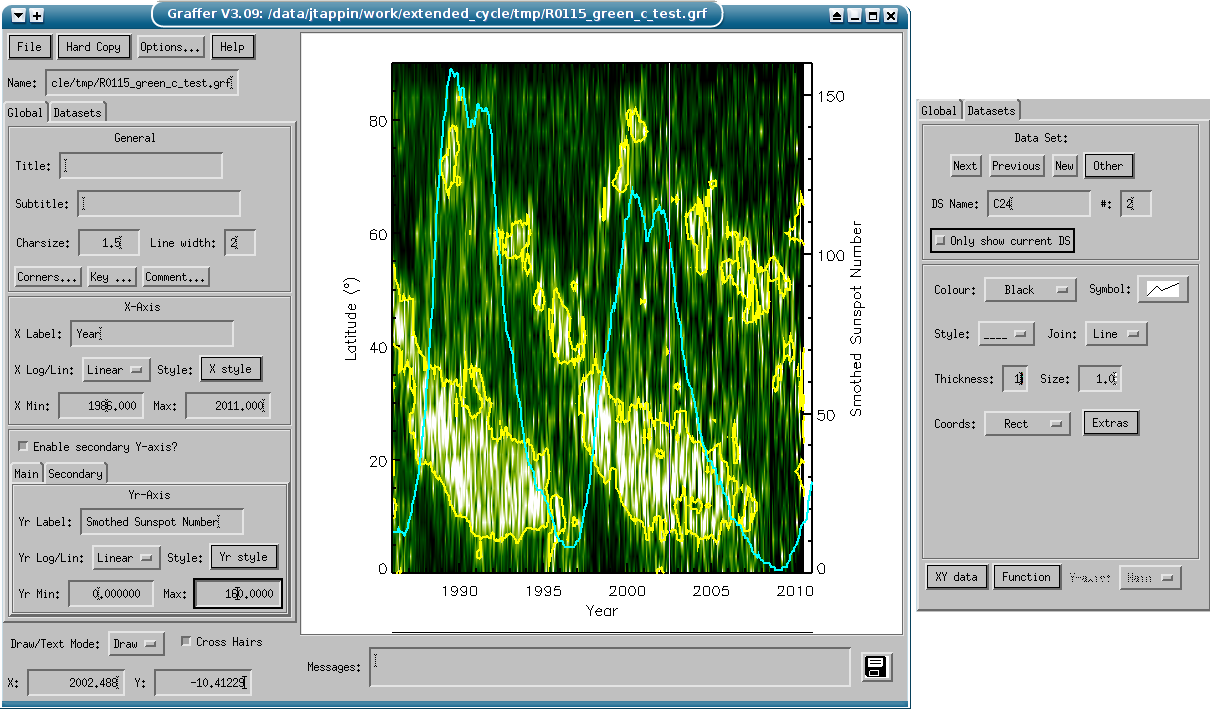
\includegraphics[width=\textwidth]{main}
  \caption{The layout of the main GRAFFER window. (With the dataset tab
    shown to the right).}
  \label{fig:main}
\end{figure}
Now that you've got GRAFFER running and a file selected, you should see
the main GRAFFER window. Depending on which mode you are operating in,
it should look like \textsc{\autoref{fig:main}}.  The main areas of the
window are:

\begin{description}
\item [Main~plotting~window:]This is where the plot is drawn. For
  suitable datasets you can operate on the data using the mouse in the
  plotting window.
\item [Utility~control~menu:]This is at the top of the control panel
  and contains the buttons for exiting GRAFFER, saving the file,
  printing it, opening new files etc. Immediately below it is a box
  that displays the current file and directory, this cannot be changed
  by the user.
\item [General~settings:]The settings which apply to the whole plot
  (title, positioning etc) are set from the {}``General settings'' box,
  which is just below the utility controls.
\item [Axis~settings:]The two axis settings boxes allow you to set the
  properties of the individual axes. There is one for the X and one for
  the Y axis. The secondary Y-axis is enabled by the checkbox button,
  and the settings for it are in the secondary tab.
\item [Dataset~control:]In the alternate tab (shown separately to the
  right of \textsc{\autoref{fig:main}}) are most of the items which are
  concerned with selecting datasets, loading data and setting the
  format of the trace.

\item[Information boxes] Below the main plot window are two small boxes
  showing the current cursor location when it is inside the plot window
  and a larger box that contains a description of the function of the
  widget currently under the cursor.

\item[Save] In the lower-right corner is a save button with a ``floppy
  disk'' icon that only appears when the file has been changed.
\end{description}

\section{Datasets}


\subsection{General comments}

The basic element of a GRAFFER plot is the \textsc{dataset}. A dataset
corresponds to a trace on the resulting plot. In the resulting plot all
the datasets are plotted on a single set of axes, using a single
scaling. All data-input and {}``line format'' operations operate on the
\textit{current} dataset.

There are four classes of dataset in GRAFFER, divided into two broad
types each with two sub-classes.


\subsubsection{Observational data }

An observational dataset consists of tabulated numbers which are
entered by the user in one of a number of ways (see below). The
subclasses are:

\begin{description}
\item [X-Y~data:]Also referred to as 1-D data. This is the basic
  GRAFFER dataset and consists of a set of tabulated X \& Y values with
  optional error limits.
\item [Z~data:]Also referred to as 2-D data. This is a rectangular
  array of Z values and the X \& Y values at which they are
  measured. Note that the grid must be rectangular but it need not be
  regular.
\end{description}

\subsubsection{Functions }

A function dataset is an IDL expression which can be evaluated by
GRAFFER. As with observational data, they are divided by
dimensionality.

\begin{description}
\item [1-D~functions:]A 1-D function dataset is an IDL expression which
  when fed an array returns another of the same length. {[}There is
  also a special case of parametric function datasets where two
  expressions are needed.{]}
\item [2-D~functions:]A 2-D function, takes 2 1-D arrays as its input
  and returns a 2-D array.
\end{description}
Note that for any dataset other than the first, the dataset must first
be created see below (p.~\pageref{make-new-ds}).


\subsection{Entering 1-D observational data\label{enter-1d}}

The usual methods of entering observational data are accessed via the
\textsc{X-Y data} pulldown menu.

\begin{table}[!ht]

  \caption{\label{ecodes}\textit{The error-bar codes in dataset files.}}

  \begin{center}
    \begin{tabular}{|l|cccc|c|}
      \hline 
      Code&Col 3&Col 4&Col 5&Col 6&Default?\\
      \hline
      \textit{none} & - & - & - & - & 2 \\
      \#Y&$\pm Y$&-&-&-&3\\
      \#X&$\pm X$&-&-&-&\\
      \#YY&$-Y$&$+Y$&-&-&4\\
      \#XX&$-X$&$+X$&-&-&\\
      \#XY&$\pm X$&$\pm Y$&-&-&\\
      \#XYY&$\pm X$&$-Y$&$+Y$&-&5\\
      \#XXY&$-X$&$+X$&$\pm Y$&-&\\
      \#XXYY&$-X$&$+X$&$-Y$&$+Y$&6\\
      \hline
    \end{tabular}
  \end{center}
\end{table}

\subsubsection{From a File}

First create an ASCII file with one line for each datum with value in
the order:

\begin{verbatim}
  X Y "lower X err" "upper X err" "lower Y err" "upper Y err"
\end{verbatim}
Any or all of the error limits may be omitted. The interpretation of
the error columns is determined by an error-bars code which is a line
starting with a hash (\#) sign and then the appropriate combination of
\texttt{X}'s and \texttt{Y}'s. The possible values are described in
\textsc{\autoref{ecodes}}. The preferred extension of the file name is
\texttt{.dat}.

To read the file, select the {}``\texttt{From file...}'' option of the
{}``\texttt{XY data}'' pulldown. This will generate a file-selector
widget which you can use to select the file. When you have the file you
want, click on the {}``\texttt{OK}'' button.

N.B. If the dataset already contains values these will be
\textbf{replaced}; if the dataset is a function then a warning is
given.


\subsubsection{From IDL top-level variables }

Rather than writing the values from a program out to a file and then
reading the file back into GRAFFER it is easier simply to transfer the
variables straight from IDL's \texttt{\$MAIN\$} program level into
GRAFFER. If you need to get variables from some other level into a
GRAFFER plot, you should use \texttt{GRAFF\_ADD}
(\textsc{\autoref{sec:graff_add}}). 

This is done via the {}``\texttt{top level variables}'' option of the
{}``\texttt{XY data}'' pulldown. This will produce a pop-up in which
you can enter the names of the variables (or slices) for X, Y and such
error bars as are appropriate. Each entry box also has a
\texttt{Pick...} button that allows you to pick from the available
variables.

The error-bar option is selected via a pull-down menu at the bottom of
the panel, this selection should be made before you have entered the
names as this controls which entry boxes are enabled. You should enter
a name or slice in each enabled box (the X box may be left empty in
which case the index is used).

When you have set all the fields that you want, click on the \texttt{Do
  it} button. If you have specified variables or slices with
incompatible lengths, then an error message will be generated and you
will be asked to try again.

N.B. If the dataset already contains values these will be
\textbf{replaced}; if the dataset is a function then a warning is
given. If a dot (\texttt{.}) is given for any of the variables, then
that variable is retained from the current state of the dataset.

A slice is an array subscript or structure tag. Array subscripts must
be constants (i.e.\ they may not contain references to other
variables). They may however reference system variables and intrinsic
functions. Examples:
\begin{description}
\item [\texttt{[0:8]}] : Legal
\item [\texttt{[1,*,4]}] : Legal
\item [\texttt{[5:*]}] : Legal
\item[\texttt{(*,0)}] : Legal, but deprecated---obsolete subscript
  delimiters.
\item [\texttt{[0:n\_elements(x)-1]}] : Illegal---contains a reference to
  a variable. 
\item [\texttt{[locs]}] : Illegal---contains a reference to a variable.
\item [\texttt{[0:n\_elements(!p.multi)]}] : Legal---but rather silly.
\item [\texttt{(0,*]}] : Illegal---mismatched delimiters.
\end{description}

Only the total number of elements in the variable or
slice is significant. If the X variable is a scalar (or 1-element
array) and Y has more elements, then X is treated as a stride length.

If it is appropriate, then variables from other levels may be selected
by prefixing the variable name with the level number followed by a
backslash (e.g.\ \texttt{2$\mathtt{\backslash}$x}, N.B. there must not be a
space after the backslash). This is really only useful (and the chooser
only accesses it) if GRAFFER is called from another procedure with the
\texttt{/BLOCK} keyword specified---in other cases only internal
GRAFFER routines are in the call stack.

Undefined variables, strings, object references and entire structures
cannot be plotted. Pointers are automatically dereferenced (before and
after slice extraction). If a complex variable is specified, only the
real part is used.

\subsubsection{Via the data editor }

If you have the values on a piece of paper (some of us still
occasionally make measurements manually and write them down in a
notebook), or if you want to remove some bad values from a dataset then
you can use the dataset editor.

The {}``\texttt{Edit values}'' option of the {}``\texttt{XY data}''
pulldown invokes the data editor. This is just an IDL text widget in
which the values in the current dataset are displayed. The normal
selection, cutting etc.\ apply.

Below the editor window is a pulldown to select the error limit
interpretation.  Only those options appropriate to what GRAFFER
\textit{thinks} is the number of columns are actually selectable. This
may not correspond with the actual number of columns---if this happens
either enter a carriage return after the last line or press the
\texttt{do it} button (in the latter case a warning message will
replace the displayed dataset for 5 seconds) and the available error
options will be updated, the current value will be set to the default
for the number of columns.


\subsubsection{With the mouse}

This method
useful for removing bad data or for indicating features displayed in a
2-D dataset. This method of editing a dataset is potentially dangerous,
and is disabled by default (you can change the default via the
\texttt{Options...} menu option) and can be enabled for individual
datasets via the \texttt{Extras} menu in the dataset tab.

The three mouse buttons each have a function (this is where the
assumption that you have a 3-button mouse comes in):

\begin{description}
\item [Left:]Enter a point: for a dataset without errors a point is
  entered at the position of the cursor; for a dataset with errors the
  dataset editor (above) is invoked with the selection point at the end
  of the dataset. The position is set at the \textbf{release} of the
  button. When the button is pressed, if there is already at least one
  point in the dataset then the cross-hairs are replaced by a line
  showing the new segment. 

  If the \textsf{ctrl} key is down when the mouse button is pressed and
  the cursor position is within 5 pixels of a line segment, then the
  point is inserted between the endpoints of that segment (in the
  unlikely event of the point being within 5 pixels of more than one
  segment, then the closest is chosen).

  If the \textsf{shift} key is down when the mouse button is pressed
  then the point will be added at the end of the dataset nearer to the
  cursor location (this allows you to prepend points).

\item [Centre:]Edit a point: for a dataset without errors the point
  nearest to the cursor when the button is pressed is moved to the
  location of the cursor when the button is released; for a dataset
  with errors the dataset editor is invoked with the pointer at the
  point nearest to the cursor. N.B. As a safety precaution, the cursor
  must be within 5 pixels of the point. When the button is pressed then
  the cross-hairs are replaced by a line showing the updated
  segment(s).
\item [Right:]Delete a point: the point nearest the cursor when the
  button is released is deleted.  N.B. As a safety precaution, the
  cursor must be within 5 pixels of the point. A circle is drawn around
  the point to be deleted if one is in range.
\end{description}
If \textsf{ctrl} or \textsf{shift} is held down when the button is
released, then the action will be cancelled. N.B.\ this means that for
inserting or prepending points, you must release the modifier key
before releasing the mouse button.

\subsubsection{A note on limits}


In many situations in the real world, some of the values in a dataset
are upper or lower limits. To plot limits requires that the dataset be
defined with asymmetrical error bars. If the value is a lower limit,
then set the \textbf{upper} error to \texttt{Inf} (The IEEE
$\infty$ value), for an upper limit, set the \textbf{lower} error to
\texttt{Inf}.

\subsubsection{Copying another dataset}
\label{sec:xycopy}

If the \texttt{Copy ...} option is selected, then a menu will give you
a choice of existing XY datasets to copy to the current dataset. By
default if the current dataset contains data, then only those of the
same type are offered, but this can be overridden by selecting the
``Show all'' button. A warning will be given before attempting to
overwrite functions or 2-D data.

This is useful (for example) if you have a dataset that you want to
plot over an image display, and you need black and white dashes to make
it show up; in that case you could set the original to black continuous
and then make a copy and display that with white dashes.


\subsection{Entering 2-D observational data\label{enter-2d}}

The entry of 2-D data is somewhat more restricted that 1-D because:

\begin{enumerate}
\item A dataset editor for 2-D data would be too unwieldy
\item Mouse editing of 2-D data is clearly not feasible.
\end{enumerate}
Therefore there are only three ways to enter 2-D data, all of which are
reached via the \texttt{2-d datasets} sub-pulldown of the \texttt{XY
  data} pulldown.


\subsubsection{From top-level variables }

This is very like the 1-D case and is reached via the \texttt{Top level
  variables} option of the \texttt{2-D datasets} pulldown. The
resulting pop-up menu has three slots for the Z, X \& Y variables (and
selector buttons.  Z must be an $(n\times m)$ array and the X \& Y must
(if given) be respectively an $n$ or $(n\times m)$-element and an $m$
or $(n\times m)$-element array; if either or both is not given then the
index number is used. Any degenerate dimensions are ignored, so a
$(n\times 1 \times m)$ array will work (e.g. if you selected slice
\texttt{[*,5,*]} from a 3-D array).

If the X or Y variable is a scalar (or 1-element array) and Z has more
elements in that dimension, then that variable is treated as a stride
length. If a dot (\texttt{.}) is given for any of the variables, then
that variable is retained from the current state of the dataset.

\subsubsection{From a file}

Again very similar to the 1-D case but the rules for laying out the
file are different in that some {}``header'' information is needed.
The format of the file:

\begin{itemize}
\item Line1: 2 numbers giving the number of X and Y values ($n_{x},\,
  n_{y}$). If $n_x$ is negative, this means the X array is
  2-dimensional, and if $n_y$ is negative then the Y array is
  2-dimensional.
\item The $n_{x}$ or $n_x \times n_y$ X values. These may be spread
  over any number of lines, but there must be the correct number and a
  new-line at the end.
\item The $n_{y}$ or $n_x \times n_y$ Y values. These may be spread
  over any number of lines, but there must be the correct number and a
  new-line at the end.
\item The $n_{x}\times n_{y}$ Z values. Again they may be spread over
  any number of lines, but there must be the correct number of values.
\end{itemize}
Note that there are no error bars on 2-D datasets.

\subsubsection{Copying another dataset.}
\label{sec:zcopy}

Again very similar to the 1-D case. There is however no ``Show all''
button as there is only one type of 2-D dataset.

\subsection{Entering functions\label{enter-fun}}

Although there are several varieties of function in GRAFFER, the format
for expressing them and the editor used to enter them are very similar
for all types. The various function editors are reached via the
\texttt{Function} pulldown which is found adjacent to the \texttt{XY
  data} pulldown.


\subsubsection{The Editors }

The four types of function can all be entered via one of the function
editors. These all share the following fields:

\begin{description}
\item [Function:]A box or boxes in which to enter the function. This
  must be a valid IDL expression which returns an array of the same
  size as its input argument.
\item [Axis~Range:]two or four boxes to enter the limits over which the
  function is to be evaluated. If no values are entered, then the range
  of the axis of the independent variable is used.
\item [Number~of~evaluations:]One or two boxes to the GRAFFER how many
  time to evaluate the function over its range (the default for this is
  25, but for straight lines you only need 2 while very wiggly
  functions may need many more).
\item [Do~it~\textmd{and}~Cancel:]Self-explanatory, the \texttt{Do it}
  button accepts the new function definition and the \texttt{Cancel}
  button rejects it.
\end{description}
The precise details vary according to the type of function being
specified:

\begin{description}
\item [\texttt{y~=~f(x):}]This is the obvious type of 1-D function. The
  function entered in the function box should be an IDL expression with
  \texttt{x as} the independent variable e.g.:

\begin{verbatim}
  sin(x)
  3.2{*}x^2 - x + !pi
  replicate(5.1,n_elements(x))
\end{verbatim}
\end{description}
Note that this last case is necessary as the obvious \texttt{5.1} does
not return an array\footnote{I suppose you could use \texttt{{[}5.1,
    5.1{]}} but then if you reset the number of evaluations you'd be up
  a gum tree (at least temporarily).}.

\begin{description}
\item [\texttt{x~=~f(y)}:]Very similar except that now x is expressed
  as a function of y so the independent variable should now be
  \texttt{y} e.g. \texttt{exp(-y\textasciicircum{}2) - 0.5}.
\item [\texttt{x~=f(t)~\&~y~=~g(t)}:]Also referred to as a parametric
  function. There are several important points here:

  \begin{itemize}
  \item There are now two function boxes to be filled, the first gives
    x as a function of t and the second gives y as a function of t. For
    example to draw a unit circle (or part thereof; see below) you
    would need to set the functions as: \texttt{sin(t)} \&
    \texttt{cos(t)}.
  \item The range of evaluation \textbf{must} be given as the parameter
    is not linked to an axis and so there is no natural boundary. The
    default is to go from 0 to 1.
  \end{itemize}
\item [\texttt{z~=~f(x,y)}:]The 2-D function entry. This requires a
  function of both X and Y to be given. Examples would be:

\begin{verbatim}
  x * sin(y)
  -1./sqrt(((x+.5)^2+y^2)>1e-6) - .5/sqrt(((x-1)^2+y^2)>1e-6) - (x^2 + y^2)
\end{verbatim}
\end{description}
In this latter case, note the use of the limiting operators to flatten
out the singularities which will, if they lie at an evaluation point,
cause GRAFFER to crash. Internally, the \texttt{x} and \texttt{y}
arrays are converted into 2-D arrays so that the examples above do
return the proper 2-D array of z-values.

As there are two independent variables, there are two sets of limits
and two evaluation counts. If you are on a system with limited memory,
remember that the function evaluation requires (at least) 3 arrays of
double precision numbers with $N_{x}\times N_{y}$\ points.

\subsubsection{Copying another function}
\label{sec:fcopy}

The \texttt{Copy ...} option allows you to copy an existing function
dataset to the current. As is generally the case a warning is given
before overwriting incompatible datasets. If the current dataset is a
function then by default only functions of the same kind are offered as
candidates, but the ``Show all'' button allows all functions to be
offered.

\subsubsection{Fit dataset }

Often, when you have observational or experimental data, you want to
fit a function to that data. While GRAFFER cannot provide a fully
general function fitting suite, there are facilities to fit polynomials
and other common variations:

\begin{description}
\item [Polynomial:]$y=\sum a_{i}x^{i}$
\item [Exponential:]$y=\exp(\sum a_{i}x^{i})$
\item [Logarithmic:]$y=\sum a_{i}\ln(x)^{i}$
\item [Power~law:]$y=\exp(\sum a_{i}\ln(x)^{i})$
\item [Piecewise~linear:]This is easier to explain than to write down
  mathematically. Essentially the data are fit by a series of straight
  lines (you say how many and GRAFFER determines the slopes and the
  locations of the breaks).
\end{description}
Note that the functional forms do in the case of a first-order fit
reduce to the more usual forms it's just easier to implement them the
way they are given here.

To invoke fitting firstly create a \textbf{new} dataset. Do not under
any circumstances attempt to invoke fitting with the data that you wish
to fit as the current dataset, if you do then the original data will be
destroyed!

When you select the fitting option on the function pulldown, a pop-up
control panel will appear which allows you to select which dataset to
fit and what kind of fit to do.

The default fitting style is a first-order fit which will appears as a
straight line with the current selection of logarithmic and/or linear
axes (e.g. for a log-log plot the default will be a power-law).  The
order of the fit for the {}``conventional'' forms is just the maximum
value of $i$, for the {}``piecewise linear'' fit the order is the
number of breaks (i.e. one less than the number of segments).

If you have some known bad points in the dataset, then they can be
excluded from the fit by selecting a slice using the standard IDL
syntax for slices (e.g. \texttt{(4:23)}).

The \texttt{update} button allows you to try a fit without destroying
the pop-up. By using this you can try various types of fit and select
the best. Note that the $\chi^{2}$ values quoted are meaningful in an
absolute sense only if the dataset being fitted has error bars, however
even for datasets without errors they do provide a relative measure of
the quality of the fit.


\subsubsection{Read function from file}

There is also an option to read a function from a file. This is most
likely to be used in conjunction with the option to save a dataset to a
file as a means of transferring complicated functions from one GRAFFER
file to another. Lest you should wish to write a function definition
with an editor and then read it into GRAFFER the format is:

\begin{description}
\item [Line~1]A function type code, which gives the \textbf{Dependent}
  variable, i.e. \texttt{Y}$\equiv y=f(x)$, \texttt{X$\equiv x=f(y)$},
  \texttt{XY$\equiv x=f(t),\: y=g(t)$} and \texttt{Z}$\equiv z=f(x,y)$.
\item [Line~2]The range over which the function is to be evaluated: 2
  numbers except for type \texttt{Z} where 4 are needed.
\item [Line~3]The number of function evaluations: 1 number except for
  type \texttt{Z} where 2 are needed.
\item [Line~4]The function itself, type \texttt{XY} needs a fifth line
  with the second function.
\end{description}

\subsection{Dataset selection and manipulation}

In addition to entering datasets, there are several other operations
that need to be performed on them. These {}``selection and
manipulation'' operations are described in the following
paragraphs. The controls for the operations are found at the top of the
\textsf{dataset} tab on the main window.


\subsubsection{Selection}

\begin{description}
\item [Create~new~dataset\label{make-new-ds}:]The \texttt{New} button
  on the dataset operations menu creates a new empty dataset at the end
  of the dataset list into which data or a function can be inserted.
  The same operation can be effected via the \texttt{select} option of
  the \texttt{Other} pulldown and selecting the item \texttt{<new>} in
  the pop-up menu.
\item [Select~dataset:]All operations such as reading data or changing
  linestyles are applied to the \textsc{current} dataset. Therefore you
  need a mechanism whereby you can make a given dataset current.


  The simplest mechanism is via the \texttt{next} and \texttt{previous}
  buttons which allow you cycle through the currently defined datasets.
  This is all very well for GRAFFER files with a handful of datasets,
  but for a file with many datasets (the most you are allowed to have
  is $2^{15}-1$ but I doubt if you will be seriously inconvenienced by
  this limit!) this could be rather time consuming, so there is an
  alternative method: the \texttt{Other} pulldown has an option
  \texttt{Select} which generates a pop-up menu with all the datasets
  listed with their sizes, types and names. To select the required
  dataset, just scroll the list widget (if necessary) and click on the
  line for the dataset you want. The \texttt{<new>} item at the end of
  the list has the same effect as the \texttt{New} button. The current
  selection is marked with an asterisk. The \texttt{Cancel} button
  destroys the pop-up and leaves the selection unchanged.

\item [Name:]Technically this probably belongs under the heading of
  {}``Dataset properties'' but conceptually it is better considered
  here, both because if its use and the location of its entry point.


  A dataset can have a name associated with it. This is an arbitrary
  string which is used for two purposes, firstly to identify the
  current dataset and secondly as a label on any legend or key on the
  plot.  The entry box below the dataset operations menu displays and
  also allows you to edit the name of the current dataset. (The serial
  number in the adjacent box is not editable.)

  The only constraint on the string used for the name is that if you
  intend to add a key to the plot then you need to remember that both
  for the hershey fonts (used on-screen) and for PostScript fonts (used
  in hard copy) the exclamation mark is an escape character; see the
  IDL User's Guide for more details.
\item[Only show current DS:] This toggle allows you to display only the
  current dataset (useful in complex plots). Text strings and the key
  (if one is present) are also suppressed when this is selected. If
  text mode (\textsc{\autoref{sec:text}}) is also selected, then only the
  text strings are displayed. If you try to print while this option is
  enabled, then you will be asked whether to print all the datasets or
  just the current.

\end{description}

\subsubsection{Manipulation}

In addition to the basic input and editor operations described in
\textsc{\autoref{enter-1d}-\autoref{enter-fun}}, there are a number of
operations which work on whole datasets. These operations are all
options of the \texttt{Other} button in the dataset operations menu.

\begin{description}
\item [Delete:]Delete the current dataset. There is a confirm pop-up
  before the dataset is actually destroyed. The next dataset becomes
  current, unless the dataset deleted was the last in which case the
  previous dataset becomes current.


  You cannot delete the only dataset in a file.

\item [Erase:]Delete the contents of the current dataset but do not
  remove its slot in the GRAFFER file. This can be done to the only
  dataset in a file.
\item [Sort:]Reorder the datasets. This generates a pop-up that allows
  you to select datasets and move them to a different location in the
  list. This can be useful if you want to make sure that one dataset is
  drawn before another as datasets are guaranteed to be plotted in
  sequence. It would also be useful if you wanted to make the items in
  the key appear in a more logical order.


  To use the pop-up just click on the dataset you want to move; the
  list will then be updated to remove the selected dataset and add a
  ``start'' placeholder. Then click on the dataset immediately
  \textsc{before} the new location of the dataset. This is likely to be
  the most convenient way of doing things until RSI implements
  ``drag-and-drop'' in list widgets.

  Multiple datasets may be moved in one invocation, but the ``Do it''
  button is disabled when there is an incomplete move (i.e.\ after a
  dataset has been selected but not relocated).

\item [Merge:]Join two datasets together. The merge option generates a
  pop-up menu with two selector menus each with a list of all the
  observational datasets in the file.


  To use it, first select the dataset to be extended from the left hand
  panel. This will enable all the compatible datasets in the right-hand
  panel, select the one you want to add. There are two additional
  options:

  \begin{enumerate}
  \item Sort resultant: If this option is selected, then the X-axis of
    the resulting dataset will be sorted.
  \item Delete appended: If this is selected, then the second dataset
    is deleted from the file.
  \end{enumerate}
  The \texttt{Cancel} and \texttt{Do it} buttons have the expected
  meaning.

\begin{quote}
  \textsf{\textbf{HINT:}} \textsf{To make a dataset consisting of two
    existing datasets, while retaining both the originals: create a
    {}``New'' dataset and then merge each of the existing datasets into
    that dataset.}
\end{quote}
\item [Write~to~file:] Write the current dataset to an ASCII file in a
  format that can be read by the \texttt{Read from file} options of the
  data and function entry menus. A pop-up will appear to allow you to
  specify the filename and directory. If you attempt to overwrite an
  existing file a confirm menu will appear to allow you to {}``back
  out''.
\item[Copy:] Make a new dataset which is a copy of the current
  dataset. The data values and type are copied. For functions the
  functions and evaluation range are copied. Display properties will be
  the defaults. The new dataset becomes current.
\item[Export:] Export the current dataset to top-level IDL
  variables. This is only available for data datasets, not for
  functions. The variable names may be set via a pop-up menu. The
  default values are listed in
 \textsc{\autoref{tab:export-names}}. 
\end{description}
\begin{table}
  \centering
  \caption{\textit{Variable names for Exports}}
  \begin{tabular}{lll}
    \hline
    Quantity & Name & Types \\ \hline
    X variable & GR\_X & All \\
    Y variable & GR\_Y & All \\
    Z variable & GR\_Z & 9 \\
    Y errors & GR\_Y\_ERR & 1,5,7 \\
    Y upper error & GR\_Y\_ERR\_U & 2,6,8 \\
    Y lower error & GR\_Y\_ERR\_L & 2,6,8 \\
    X errors & GR\_X\_ERR & 3,5,6 \\
    X upper error & GR\_X\_ERR\_U & 4,7,8\\
    X lower error & GR\_X\_ERR\_L & 4,7,8\\
    \hline
  \end{tabular}
  \label{tab:export-names}
\end{table}
To select which Y-axis to use (when a secondary Y-axis is enabled),
there is a pulldown menu adjacent to the input options.

\subsection{Display style}


\subsubsection{1-Dimensional data}

Most of the IDL style options for plot traces are available. These are
set with the various entry windows and pull down menus below the plot
window. Note that these options are identical for functions and for
observational data.

\begin{description}
\item [Symbol:]The symbol to use for plotting the points. The pull down
  menu has images of the symbols, and displays the current one on the
  undisturbed button. The default is a continuous plot. There are now
  several extra symbols beyond the default IDL symbol set.
\item [Join:]Set the type of line to join the points. This can be
  straight lines joining the points, a histogram type line or no line
  at all.  Note that no symbol and no line is allowed and will result
  in the trace becoming invisible.
\item [Size:]The size to use for the plotting symbols as a multiple of
  the default size. This is ignored for continuous or histogram plots.
  Any floating point value is accepted. The symbol size also determines
  the length of the caps on error bars.
\item [Line~style:]Line style to use for continuous plots, ignored for
  discrete symbols. The pull down menu shows the available
  styles. Error bars are always drawn with solid lines.
\item [Line~thickness:]The width of the line in terms of the basic line
  width. Enter any real value ($>0. \& \leq100.$) to set the width. This is used
  both for continuous plots and for discrete symbols. Note that at
  least on the printers I use, there is very little visible difference
  between a thickness of 1 and of 2.
\item [Colour:]The colour is set via a pulldown. Most colours have
  names, but some for which I couldn't think of a description are given
  as an RGB triple. There is a difference between \texttt{omit} and
  \texttt{white}: in the first case, the trace is simple not drawn at
  all; in the second, it is drawn in the background colour which will
  overwrite earlier traces and also take time. If ``Custom'' is
  selected, then a pop-up menu allows you to define a colour using
  sliders or entry boxes.
\item [Coordinates:]The pull down allows you to select one of three
  coordinate systems:

  \begin{description}
  \item [Rectangular:]The usual X-Y plots.
  \item [Polar~(rad):]Data are $\mathrm{r}$ and $\theta$ values with
    the angles being given in radians.
  \item [Polar~($^{\circ}$):]As above but the angles are given in
    degrees.
  \end{description}
  When the system is changed, the interpretation of the values changes,
  the values themselves are unaltered.

\item [Extra~options:]The \texttt{Extra} button generates a pulldown
  that allows the toggling of some special options:

  \begin{description}
  \item [X-axis~sorting:]For continuous plots, it is possible to
    request that GRAFFER sort the x-axis points into ascending order
    before plotting them. This is controlled by a 2-valued pull down
    menu. Obviously it has no visible effect if discrete symbols are in
    use.
  \item [Clipping:]Normally IDL clips plots at the axis box, however
    there are times when it is desirable to let a plot go over the
    box. To do this switch the \texttt{Clip to box} option to
    \texttt{Off}.
  \item [Mouse~editing:]For observational data it is usually possible
    to enter, modify and delete points using the mouse, however this
    may not be desirable so is disabled by default; you can use the
    \texttt{Mouse editing} option to allow the current dataset to be
    changed with the mouse.
  \end{description}
\end{description}

\subsubsection{2-Dimensional data}

For 2-D data there are far fewer options as to how to plot the data
than there are for line plots. The display options are now collapsed to
a single button which allows you to toggle between contours and an
{}``image'' format.  In each case, the menu below the choice allows you
to set the detailed options.
\begin{figure}[htbp]
  \centering
  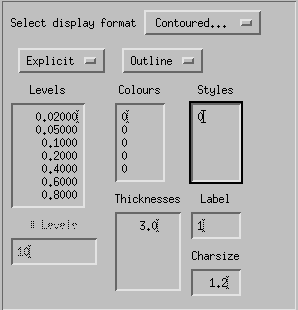
\includegraphics[width=0.4\textwidth]{main-ds3a}~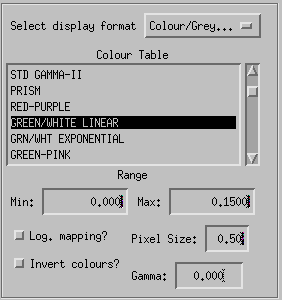
\includegraphics[width=0.4\textwidth]{main-ds2}
  % 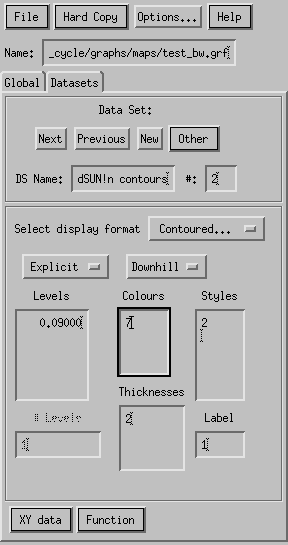
\includegraphics{contour}
  \caption{The datasets panel with (left) contouring options and
    (right) colour/greyscale options shown.}
  \label{contour}
\end{figure}
\begin{description}
\item [Contoured~display:]The contouring menu
  (\textsc{\autoref{contour})} allows you to specify all the options
  that can be used in a contour plot.

  \begin{description}
  \item [Levels:]The levels can be either explicit, in which case the
    \texttt{levels} entry box is enabled as in
    (\textsc{\autoref{contour})} and levels can be entered one per
    line. The sorting of the levels into increasing order as required
    by the CONTOUR procedure is handled by GRAFFER.


    To use a given number of equi-spaced levels, use the pulldown in
    the top left to select \texttt{Implicit levels}, this will disable
    the levels box and enable the \texttt{\# Levels} box in which you
    can enter how many contour levels you want. This doesn't use IDL's
    internal level setting routines as they do not allow all of the
    other options, so it is done by GRAFFER\footnote{For real enthusiasts, the levels are determined as
      \texttt{levels = rg {*} (findgen(nl)+.5)/nl + mn} where
      \texttt{rg} is the range of the data (ignoring infinities \&
      NaNs), \texttt{mn} is the smallest value in the data and
      \texttt{nl} is the number of levels.}.

  \item [Colours:]Specify the colours of the colour lines (or fill if
    requested).  Unlike the colour settings for line plots, these are
    given by index, the interpretation of the indices is given in%
    \begin{table}[!ht]

      \caption{\textit{\label{col_index}The GRAFFER colour indices.}}

      \begin{center}
        \begin{tabular}{|c|rrr|l|}
          \hline 
          Index&      Red&      Green&      Blue&      Name\\
          \hline 
          0&      255&      255&      255&      White (BG)\\
          1&      0&      0&      0&      Black (default)\\
          2&      255&      0&      0&      Red\\
          3&      0&      255&      0&      Green\\
          4&      0&      0&      255&      Blue\\
          5&      0&      255&      255&      Cyan\\
          6&      255&      0&      255&      Magenta\\
          7&      255&      255&      0&      Yellow\\
          8&      255&      127&      0&      Orange\\
          9&      127&      255&      0&      \#7f ff 00\\
          10&      0&      255&      127&     \#00 ff 7f \\
          11&      0&      127&      255&    \#00 7f ff \\
          12&      127&      0&      255&     \#7f 00 ff \\
          13&      255&      0&      127&      Mauve\\
          14&      85&      85&      85&      Dark Grey\\
          15&      170&      170&      170&      Light Grey\\
          16 & 170 & 0 & 0 & Dark Red\\
          17 & 255 & 85 & 85 & Light Red\\
          18 & 0 & 170 & 0 & Dark Green\\
          19 & 85 & 255 & 85 & Light Green\\
          20 & 0 & 0 & 170 & Dark Blue\\
          21 & 85 & 85 & 255 & Light Blue\\
          22 & 0 & 170 & 170 & Dark Cyan\\
          23 & 85 & 255 & 255 & Light Cyan\\
          24 & 170 & 0 & 170 & Dark Magenta\\
          25 & 255 & 85 & 255 & Light Magenta\\
          26 & 170 & 170 & 0 & Dark Yellow (brown)\\
          27 & 255 & 255 & 85 & Light Yellow\\
          \hline
        \end{tabular}
      \end{center}
    \end{table}
    \textsc{\autoref{col_index}}. If the number of colour indices given
    is less than the number of levels plotted, then the indices are
    recycled.
  \item [Thickness:]Specify line thicknesses for the contours.
  \item [Styles:]Specify the linestyles for the contour lines. These
    are the standard IDL linestyles, described in the PLOT keywords
    documentation.
  \item [Filled/Outline:]This pulldown allows you to specify filled
    contours.  With a suitable selection of colours this can be a very
    effective way of displaying data but for large datasets it is slow.

\begin{quote}
  \textsf{\textbf{HINT:}} \textsf{There is a dirty way to get a
    {}``Stepped greyscale'' effect. Firstly ensure you have the
    greyscale colour table loaded by GRAFFER (this is not the same
    thing as using LOADCT, 0; display the data in {}``Image'' format
    and select the grey table there) and then use colour indices
    selected in the range 16-143.}
\end{quote}
\item [Labelling:]IDL allows the labelling of selected
  contours. GRAFFER doesn't allow the full functionality but allows you
  to label every $n^{\mathrm{th}}$ contour. Specifying 0 means don't
  label any contours.
\item[Charsize] The character size to use for contour labels (relative
  to the default).
\end{description}
\item [Colour/Greyscale~display:]Also referred to as {}``Image''
  display.  To do this, the dataset is warped to fit the data
  coordinate system and the resulting image is displayed. While this
  can make a nice display it has two serious drawbacks:

  \begin{enumerate}
  \item It is slow, seriously slow on a small machine.
  \item It completely obscures all earlier datasets.
  \end{enumerate}
  When this option is selected, then the {}``image'' options menu
  (\textsc{\autoref{contour}}) is displayed. The options are rather
  simpler than those for a contour plot:

  \begin{description}
  \item [Range:]The range of values to map from {}``black'' to
    {}``white''.  If these are both zero, then the minimum and maximum
    of the data are used.
  \item [Colour~table:]Select any of the available colour tables; when
    the menu appears, the current table will be shown highlighted.
  \item [Gamma:]The power-law to use in mapping colour indices to the
    data values (see the LOADCT \& XLOADCT documentation). In essence a
    value of $\Gamma$ less than 1 puts most of the colours at the lower
    end of the data range.
  \item [Pixel~size:]Because GRAFFER has to warp the dataset to fit the
    data coordinate system, it has to create an image array with a
    colour index for each pixel covered by the {}``image''; this is all
    very well on a screen with typically 0.28~mm pixels but for
    PostScript with its flexible pixel size the notional pixel size is
    very small and hence the resulting image would be huge. To avoid
    this problem, you can specify a notional pixel size to be used in
    making hard copy.  The size is given in mm and the default of
    0.5~mm is usually adequate.
  \item[Log mapping?] Select whether to map the colours
    logarithmically. Note that this will only work with a
    positive-definite dataset or explicit range with both limits
    positive.
  \item[Invert colours?] Select whether to map the colours with the
    high values at the dark end of the table.
  \end{description}
\item[Hidden:] If this is selected, then the dataset is not
  displayed. There are no options.
\end{description}

\section{File-wide settings}

While the options discussed in the preceding pages have applied only to
specific datasets, others apply to the whole file. These options are
set from the \textsf{general} tab to the left of the main plotting
window.


\subsection{General settings}


\subsubsection{Plot annotation}

The plot titles and subtitles can be entered in the appropriate boxes
at the top of the general settings menus. The only subtlety to be aware
of is the IDL plotting string escape sequences (see the IDL User's
Guide) for specific details. To prevent excessive error messages, the
plot is not updated if any annotation string ends with a single
exclamation mark.


\subsubsection{General style}

The character size and line width settings allow you to specify:

\begin{enumerate}
\item The character size for all annotations (the relation between the
  sizes of the title, subtitle and axis labels is defined by IDL and
  GRAFFER does not try to change these (it can be done but the defaults
  are pretty good and it would be a horrible job to fit in all the
  extra setting boxes).
\item The line thickness used for the axes (again in principle you
  could set the axis line widths separately but it would usually be
  ugly and there isn't room for the controls).
\end{enumerate}

\subsubsection{Geometry}

For most purposes IDL's default plotting region is perfectly adequate,
and that is what GRAFFER uses by default. However there are occasions
when you need more precise control of the shape of the plot and the
size of its margins. If and when you do need this capability, the
\texttt{Corners...} button generates a pop-up menu to set these
options.

There are two ways of specifying the plot geometry:

\begin{description}
\item [By~region:]This sets the corners of the axis box in normalized
  coordinates. To use this select the \texttt{Corners} option on the
  pulldown at the top of the menu and enter the x \& y coordinates of
  the lower left and upper right corners in the boxes. The \texttt{Do
    it} button will not be enabled until the values are legal, so you
  can't crash it!
\item [By~aspect~ratio:]This uses David Fanning's ASPECT routine to
  define the corners such that the aspect ratio of the plot is
  preserved even if it is sent to different shaped pages. To use this
  select the \texttt{Aspect ratio} option of the top pulldown and enter
  the aspect ratio (defined as the length of the Y axis divided by the
  length of the X axis) and a margin size. The margin size is expressed
  as a fraction of the page size, and this is interpreted such that the
  smaller margin will be that large and the other will be as large as
  needed to achieve the required aspect ratio.
\item[Isotropic:] Enabling this check box, forces the scales on both
  axes to be identical. The actual sizing of the plot then uses IDL's
  defaults. This option is not available when a secondary Y-axis is
  enabled.
\item[HC Aspect Ratio:] Enabling this check box tells GRAFFER to
  display the plot on the screen with the same aspect ratio as it will
  have in the final hard copy. (This is independent of the other
  settings).
\end{description}
To restore the default margin settings, invoke the pop-up and click on
the \texttt{Defaults} button


\subsubsection{Key or legend}

Plots with several traces on them are often useful, but without some
explanation no-one other than the person who drew the plot will know
what the traces are. For this reason GRAFFER provides a mechanism for
adding a key to the plot.
\begin{figure}[htbp]
  \centering
  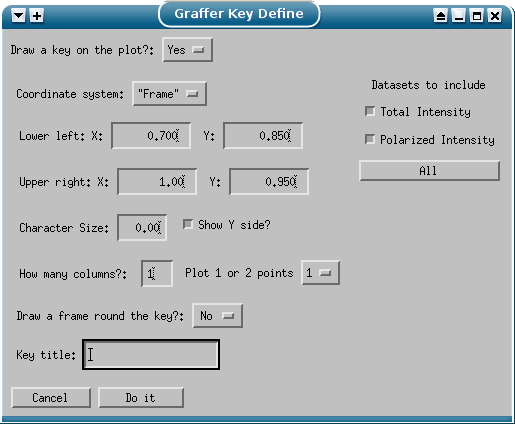
\includegraphics[width=10cm]{key}
  \caption{The key (or legend) definition menu of GRAFFER.}
  \label{key menu}
\end{figure}

Pressing the \texttt{Add key} button creates the key definition pop-up
(\textsc{\autoref{key menu}}). The first time you invoke this (for any
given GRAFFER file), the menu will be disabled apart from the
\texttt{Draw a key on the plot?} pulldown at the top; only when that
pulldown is set to \texttt{Yes} does the rest of the menu become
accessible. The menu can conceptually be split into two halves. The
left-hand side specifies the properties of the key while the right
specifies which datasets are to be included.

The location of the menu is specified by giving the coordinates of the
lower left and upper right corners in one of three coordinate
systems\label{coordsys}:

\begin{description}
\item [Data:]The coordinates are given in the same coordinate system as
  the data being plotted. This system has the property that if you
  change the axis limits, the key will remain fixed relative to the
  traces.  If you change the plot geometry (see above), the whole plot
  will change in a self-similar way. It is often difficult to figure
  out just what the box will look like especially in logarithmic
  plots. Data coordinates always use the primary Y-axis.
\item [Normalized:]The coordinates are given in coordinates which run
  from $(0,0)$ in the lower left corner of the page to $(1,1)$ in the
  upper right corner of the page. This means that the key box is fixed
  relative to the page and will move relative to the axes if the plot
  boundaries are moved and relative to the traces if the plot limits
  are changed. Strictly these GRAFFER uses ``region'' coordinates so
  that the location is correct when hard-copy aspect ratio is selected.
\item [Frame:]This system (which is implemented by GRAFFER not by IDL)
  is similar to the Normalized system, but measured relative to the
  corners of the axis box. This means that the plot behaves in a
  self-similar way when you change the boundaries, and the key remains
  fixed relative to the axes when you change the limits. With a
  suitable boundary setting you can put the key outside the axis box by
  using coordinates outside the range 0 to 1. \textbf{This is the
    default system.}
\end{description}

If the default character size is not suitable, then it can be adjusted
by entering a scale factor in the ``Character size'' box, this is a
factor relative to the default (which depends on the size of the axes
and also the global charater size setting).

If you have a secondary Y-axis, then checking the ``Show Y side'' box
adds \texttt{(l)} or \texttt{(r)} after the description to indicate
which axis is applicable to that dataset.

You can arrange the items in the key in any number of columns (although
in practice more than 2 tends not to work very well), just enter the
number of columns you want in the box.

There are two possible formats for the line sample each of which has
advantages and disadvantages:

\begin{description}
\item [1~point:]Plot a short horizontal line segment (if there are
  lines) with a single symbol (if any) in the centre. This is the more
  compact layout and usually looks better, but it cannot distinguish
  normal lines from histogram formats.
\item [2~point:]Plot a sloping line segment with a symbol at each end.
  This needs a little more room and can look untidy but does
  distinguish sloping-line traces from histograms. For historical
  reasons this is the default.
\end{description}
The format is determined by the \texttt{1 or 2 points}
pulldown. Another pulldown determines if a box is to be drawn round the
key.

If a title is entered in the \texttt{title} box, then this is written
above the key, spanning all columns for a multi-column key.

The right-hand side of the menu is a selector menu to determine which
datasets will be listed in the key, only the 1-D datasets (observations
and functions) are listed. In addition to the buttons for the
individual datasets, there is an \texttt{All} button which selects all
the datasets (you can then deselect the ones you don't want).

Unfortunately it is not possible to provide a dynamic update to the key
on the plot, so to see what it looks like you need to click on
\texttt{Do it} and then try again if it doesn't work. Note that
datasets with a colour of \texttt{Omit} are not included even if they
are selected (but they will appear as soon as the colour is changed).


\subsection{Axis settings}

The settings for the two axes are identical and so I will only describe
a generic axis setting. Almost all of the standard IDL axis styles are
available along with a number of extensions.

\begin{description}
\item[Enable~secondary~Y-axis?] (Y-only) This check box is used to
  enable/disable the secondary Y-axis. When it is disabled, then the
  contents of the ``secondary'' tab are desensitised, as is the Y-axis
  selector on the dataset menu.
\item[Main/Secondary] (Y-only) Tabs to select whether to adjust the
  primary or secondary axis.
\item [Label:]The axis label can be entered via the label box. Remember
  that the exclamation mark is an escape character (see IDL User's
  Guide); to reduce the number of error messages, the label is not
  updated if the string ends in a single exclamation mark.
\item [Logarithmic/Linear:]This is set by a toggle pulldown.When
  logarithmic is chosen, if one of the limits (see below) is zero or
  negative, the plot will not be updated until the limit is changed.
\item [Style:]This pulldown covers a multitude of sins, including but
  not limited to the IDL {[}XY{]}STYLE key settings. Each option
  generates a further pulldown of sub-options. Where appropriate, the
  selected sub-option is indicated by an asterisk.

  \begin{description}
  \item [Exact~range:]By default IDL (and hence GRAFFER) rounds the
    axis limits to some {}``nice'' range which covers the requested
    axis range. If however you really want an exact range, this can be
    forced by setting the exact range option to \texttt{On}.
  \item [Extended~range:]If this is switched on the the axis is
    extended by a small amount (5\%) from the requested limits. This
    operates \textit{after} the any rounding.
  \item [Draw~axes:]Normally IDL draws an axis on each side of the plot
    (thus producing a full box). Both axes can be turned off by setting
    this option to \texttt{Off}.
  \item [Draw~box~axis:]Turning this option to \texttt{Off} just
    suppresses the axis to the right or above the plot. If the draw
    axes option is turned off then it has no effect. This option is
    disabled for the Y-axes when a secondary Y-axis is enabled.
  \item [Minor~ticks:]GRAFFER does not have room to provide full
    support for arbitrary control of the number of minor tick marks. If
    this option is set to \texttt{On} (the default) IDL determines the
    number of minor ticks to add, when it is \texttt{Off} then minor
    ticks are suppressed.
  \item[Annotations:] This option allows the suppression of the normal
    labelling of the axis.
  \item [Time~labelling:]Normally only used on the X-axis, but you
    might want it on Y and it's easier to provide the option than to
    omit it\footnote{Because of limitations in the way IDL uses label
      formatting functions, time labelling is not supported for the
      secondary Y-axis.}.  This option provides some support for
    labelling an axis with times.  When it is switched \texttt{On} then
    a pop-up appears to ask you the units in which the time is given,
    what is the largest unit you wish to put on the plot (e.g. if the
    values are in hours, you might want to label the axis in days and
    hours) and the label to give to the zero point (this is given in
    the largest unit displayed---the idea behind this is to allow a
    date to be added to an axis whose times are in hours of a given
    day). The largest supported unit is days.

\begin{quote}
  \textsf{\textbf{Example:}} \textsf{Suppose you have a time series
    lasting a couple of days starting on 24 February 1997 and the times
    are given in hours from 00:00 UT on 24 Feb. The you should set the
    time unit to} \texttt{hours}\textsf{, the {}``display to'' unit to}
  \texttt{days} \textsf{and the zero value to 24. You should them label
    the axis (say)} \texttt{February 1997}\textsf{.}
\end{quote}
\item [Origin~Axis:]If this option is turned \texttt{on}, then add an
  axis going through the origin of the other axis (if that is on the
  plot). If the draw axes option is off then the axis will be labelled
  with the axis label, normally it will not be labelled. For the X-axis
  this option is disabled if a secondary Y-axis is enabled. For the
  Y-axis, annotations are suppressed if an origin axis is selected for
  both Y-axes.
\item [Grid:]If this is set to a line style, then extend the major tick
  marks to form a grid and draw them with the given style.
\item [Autoscale:]This isn't really a style option as such, but a means
  of updating the axis limits (see below) to accommodate the
  data. There are two possible ways to do this:

  \begin{description}
  \item [Extend:]This will increase the upper limit, or decrease the
    lower limit so as to include all the datasets within the range.
  \item [Extend~or~shrink:]This will also raise the lower limit or
    lower the upper limit to remove blank space.
  \end{description}
  In either case for Y-axes, if a secondary axis is enabled, then only
  those datasets plotted against that Y-axis are scanned.
\item[Advanced ...] This option allows you to specify some more
  advanced options for axis labelling, via a separate menu
  (Figure~\ref{fig:adv-axis-menu}). Current
  settings available are:
  \begin{figure}
    \centering
    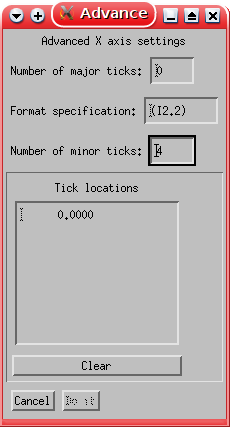
\includegraphics{axis_adv}
    \caption{The menu for setting advanced axis options.}
    \label{fig:adv-axis-menu}
  \end{figure}
  \begin{itemize}
  \item The number of major tick intervals.
  \item The number of minor tick intervals, this overrides the simple
    on/off setting of the minor ticks option above.
  \item The format for the tick annotations, this may either be a
    format string enclosed in parentheses or a formatting function
    name, the handler verifies that the string is one of: empty,
    enclosed in parentheses, an existing function or a file in the
    search path; it does \textbf{not} verify that it is a valid format
    string or formatting function.
  \item Explicitly selected major tick locations (this will override
    the number of major tick intervals).
  \end{itemize}
  Setting these to zero or an empty string will use IDL's defaults.
\end{description}
\item [Limits:]The Min and Max boxes allow you to set the axis
  range. If the range requested is invalid, then the plot will not be
  updated until a valid range is entered (this prevents GRAFFER
  crashing while you are editing the numbers). To scale the axis to the
  data, use the Autoscale option of the Style pulldown.
\end{description}

\section{Text}
\label{sec:text}

In addition to the standard plot labels and the key options, GRAFFER
also has facilities to add text at arbitrary locations on the plot.  To
use this facility, you must switch GRAFFER to text mode which makes it
interpret mouse button clicks in the plot window as text operations
instead of dataset operations. The mode button is a pulldown just below
the global and dataset tabs.  When you are in text mode, the cross
hairs that follow the cursor change from continuous to dashed and
extend over the whole window rather than just the axis box.

The button assignments are essentially the same as for the mouse
dataset editing operations, i.e. the LEFT button adds a new text item
at the location of the pointer, the CENTRE button initiates the text
editor on the existing string whose anchor point is closest to the
pointer and the RIGHT button deletes the string whose anchor is nearest
the pointer. Both the edit and delete operations have a maximum
distance of 5 pixels.
\begin{figure}[htbp]
  \centering
  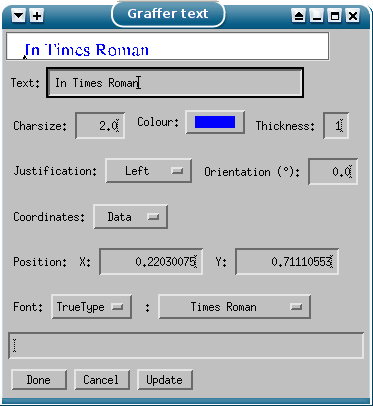
\includegraphics[width=12cm]{Text}
  \caption{The text input/editing menu of GRAFFER.}
  \label{text panel}
\end{figure}
Insertion of new text and editing of existing text are both
accomplished via the same text input pop-up (\textsc{\autoref{text
    panel}}). There are many user-settable fields in the menu:

\begin{description}
\item [The~text~string~itself:]This is a text entry widget into which
  you can type the text string to be displayed. Any of the IDL graphics
  controls ( !<\textit{char}> commands) may be used as these text
  strings are displayed in vector fonts (unless of course you have
  specifically requested hardware font). As you type the text into the
  box, it will be reflected in the graphics window above in the size,
  font etc. in which it will appear on the plot. If no text string is
  given it will be displayed as \texttt{<NULL>}, this will not be
  printed on a hard copy, nor is it displayed while editing the
  text. Also, text items after the current one may not appear while
  editing is in progress.
\item [Character~Size:]Enter a floating-point value to give the
  character size in terms of the default value. When hard copies are
  made, the size is adjusted to give the same number of characters
  across the page as were on the screen.
\item [Colour:]The colour of the text, the pulldown has the same
  colours as for plot traces, except that there is no option to omit
  the text entirely. In the figure the ``alternate'' colour pixmap
  selector is enabled. Custom colours can be defined in the same way
  as for plots.
\item [Thickness:]Enter a real value to specify the line thickness
  to be used for the character drawing. This should be used with
  caution, but the results in hard copy are usually better than the
  X-windows display suggests.
\item [Justification:]A pull down which allows you to set Left, Centre,
  Right or otherwise-justified text. For non-standard justifications a
  pop-up with a slider is used to set the justification in the range
  0.0 (Left justified) to 1.0 (Right justified).
\item [Orientation:]Set the orientation of the text. This is measured
  in degrees anti-clockwise from the normal position of parallel to the
  X-axis and going left to right.
\item [Coordinate~system:]A pull down to select Data, Normalized or
  Frame coordinates as the system in which the text is anchored. The
  default is data, but if you wish the text to remain in the same place
  on the page when you change the axis range, then use normalized, if
  you want the text fixed relative to the axes use Frame. For more
  details of the systems see p~\pageref{coordsys}.
\item[Y-axis:] If a secondary Y-axis is available, then this allows you
  to select which one to use for Data coordinates. This selector is not
  created when there is no secondary Y-axis, and is disabled when the
  coordinate system is not Data. By default, the coordinate system of
  the current dataset is selected.
\item [Position:]Set or adjust the position of the anchor point, both X
  and Y are floating-point numbers and are given in the currently
  selected coordinate system.
\item [Font:] A pair of pull downs to select the font. The first
  selects the font group, and the second the specific font. All the
  recognized fonts are available---for illustrations of the characters,
  and information on the mappings see the ``IDL User's Guide''. For
  hardware fonts, the rendering in X will prbably be incorrect and also
  the orientation will probably not be fully honoured.
\end{description}
In order to reduce the refresh time as you are typing the text string,
the plot is not updated after every character you type, instead the
string is displayed in a small window at the top of the text entry menu
(the only characteristic which is ignored is the orientation).  To see
how it will actually look on the plot, click on the \texttt{Update}
button, this will update the plot without exiting the text menu. The
\texttt{Do it} and \texttt{Cancel} buttons have their usual meanings.

Remember that when you are in text mode you cannot then use the mouse
to edit datasets, however all other dataset operations remain valid.


\section{Control}

In this section I shall describe the various {}``control'' operations
that allow GRAFFER to deal with the outside world and thus be useful.
All of the operations are controlled from the buttons on the top-left
of the GRAFFER control panel.


\subsection{Hard Copy}

GRAFFER supports the generation of PostScript hard copy files with a
wide range of options. When requesting hard copy you can retain the
current options (or the defaults if none have been set) by selecting
the \texttt{Quick} option of the pulldown. If you select the
\texttt{Set up} option, then the hard copy setup menu will be produced
(\textsc{\autoref{hardcopy menu}}).

 \begin{figure}[htbp]
   \centering
   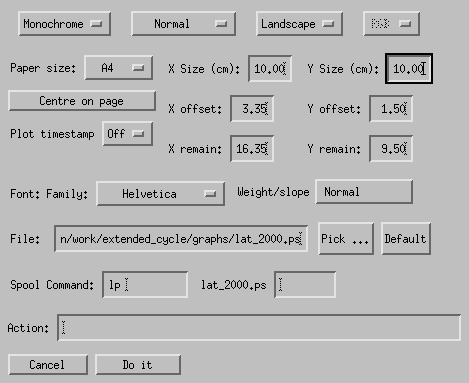
\includegraphics[width=10cm]{hardopts_ps}\vspace{5mm}
   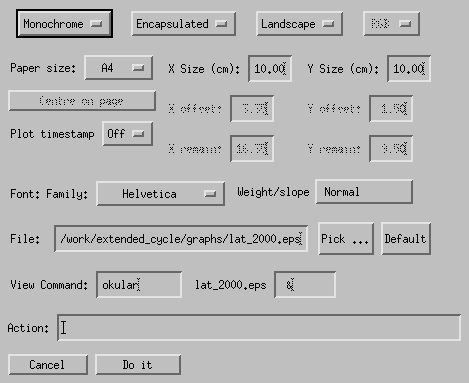
\includegraphics[width=10cm]{hardopts_eps}
   \caption{The GRAFFER hard copy set up menu. Upper: with regular PS
     selected; Lower: with Encapsulated PS selected.}
   \label{hardcopy menu}
 \end{figure}
 At the top are four pulldown toggle buttons to select:

 \begin{description}
 \item [Monochrome/Colour:]Whether to generate colour PostScript or
   not.  The default is colour. In monochrome mode, all line plots
   appear black, but 2-D data displayed in {}``image'' format will
   appear as a greyscale.
 \item [Normal/Encapsulated:]Normal is just a regular printable
   PostScript file. Encapsulated is not printable, but can be included
   into other files e.g. \texttt{xfig}, \LaTeX\ etc. The filename ends
   \texttt{.ps} or \texttt{.eps} according to the selected option. PDF
   (Print) generates a PDF file with the selected page size, suitable
   for printing, PDF (LaTeX) generates a PDF file suitable for
   including into PDF\LaTeX\ documents. Since IDL does not generate PDF
   directly from direct graphics, a PS or EPS file is generated, and
   then converted to PDF using \texttt{gs}, if \texttt{gs} is not
   installed on your system, the PDF outputs will not be available.
 \item [Landscape/Portrait:]Describes the orientation of the plot on
   the page. If encapsulated PostScript is selected then this is
   ignored apart from changing the default dimensions.
 \item[RGB/CMYK] Select which colour representation to use (disabled if
   monochrome is selected).
 \end{description}
 The size and placement of the plot can be controlled by the buttons
 and entry boxes in the next few lines of the menu:

 \begin{description}
 \item [Paper~size:]Allows you to toggle between the European A4
   ($210\times297\mathrm{mm}$) (default) and American Letter
   ($8.5\times11^{\prime\prime}$) paper sizes. As IDL doesn't put paper
   size commands into its PostScript output\footnote{This is a good
     thing as if a file with embedded paper size commands is sent to a
     printer with different sized paper it will typically hang the
     queue until someone intervenes.} this is just used in GRAFFER's
   internal accounting to figure out margins etc.
 \item [Centre~on~page:]Adjust the offsets so that the current page
   size is centred on the paper; note this is not a retained
   characteristic so you have to re-apply this any time you change the
   page dimensions. (Disabled for EPS).
 \item [X~\&~Y~sizes:]Set the X \& Y dimensions of the page. The X \& Y
   directions correspond to the directions of the axes on your plot.
   Note that there is nothing to stop you making a portrait orientation
   file with the X dimension larger than the Y, in fact this is the
   recommended way of making landscape encapsulated files.
 \item [X~\&~Y~offsets:]Set the distance between the lower left corner
   of your plot page and the lower left corner of the page. Again this
   refers to the corners as seen when you are looking at the plot in
   the usual way people look at plots, GRAFFER handles the axis
   interchanging needed (but it will get it wrong if you don't tell it
   the right paper size!). (Disabled for EPS).
 \item [X~\&~Y~remain:]These are not user settable, they just tell you
   how far the top right corner of your plotting page is from the top
   right corner of the paper. (Not meaningful for EPS).
 \end{description}
 The other {}``formatting'' options are:

 \begin{description}
 \item [Plot~timestamp:]If this is selected, then add a string with the
   date of generation and the username of the generator to the plot.
 \item [Font:]There are two pulldowns that allow you to select any of
   the PostScript fonts that IDL knows about (yes even
   Zapfdingbats!). The first selects the family and the second the
   weight and slant. This font is used for titles, axis annotations and
   labelling, keys and any text strings where hardware font was
   selected. Text strings in vector fonts are not affected.
 \end{description}

 The default output file is derived from the GRAFFER file name by
 replacing the suffix with \texttt{.ps} or \texttt{.eps} according to
 the selected output. This can be changed via the output file entry box
 or the \textsf{Pick~...} button. The default may be restored with the
 \textsf{Default} button.

 For ``normal'' PostScript files, GRAFFER will automatically spool
 the file to the printer. The default command is \texttt{lp}, this can
 be changed by entering a new command in the ``Spool command'' boxes:
 the first box is for that part of the command which precedes the
 filename and the second for anything that has to come after the
 filename\footnote{Originally this was intended for VMS where options
   such as the print queue name came after the file name.}. When
 encapsulated output is selected, then a PostScript viewer is selected.

\begin{quote}
  \textsf{\textbf{Example:}} \textsf{Suppose, you have a printer that
    needs some special file to be attached to the file to make
    transparencies so that the command to spool} \texttt{foo.ps}
  \textsf{is:}
  \begin{verbatim}
    cat upper.ps foo.ps | lp -dEaf-color1
  \end{verbatim}
  \textsf{then the two boxes should contain respectively:}
  \begin{verbatim}
    cat upper.ps
    | lp -dEaf-color1
  \end{verbatim}
\end{quote}
The \texttt{Cancel} and \texttt{Do it} buttons have their usual
meanings.


\subsection{Saving and dumping}

One of the key features of GRAFFER is that you can save you plot to a
file and then come back to it later. The various saving options are
under the \texttt{File} menu, there is also a sub-menu to allow you to
make screen dumps.

There are three save options which allow you to save to the current
file in the current format or to save to a specified file in either
binary or ASCII format. Clicking on the {}``Changed'' indicator on the
far right of the control panel does a save to the current file, in the
current format.

Normally binary files are preferable as they are smaller and quicker to
read and there is no risk of losing precision in floating point
numbers. However if you want to transfer the file to a different
platform then you should use ASCII as the representations of the
numbers may differ\footnote{Unfortunately I was not able to devise an
  automatic means of distinguishing binary, ASCII and non-GRAFFER files
  if I used XDR for the binary form.  Abandoning ASCII would have meant
  that version 1 could not be read into version 2. For machines with
  IEEE floating point formats (most machines nowadays) binary files can
  be read irrespective of endianness by the simple expedient of
  checking the version number and swapping bytes if the raw version
  number is greater then 255.}.

If you request a save to a new name, a pop-up will appear to allow you
to edit the new filename. If you try to save over an existing filename,
a warning will be given and you will have the option of overwriting or
trying another name.

The screen dump allows you to dump the GRAFFER plot window to a PNG,
TIFF or NRIF file, the name will be the current filename with an
appropriate extension. JPEG is not available as it is a lossy scheme
unsuitable for line plots. There is also an option to start the IDL
image save dialogue to choose any format known to IDL\footnote{At least
  on my installation, although Jpeg2000 is theoretically available it
  does not actually work.}.


\subsection{Opening a new file}

When you start GRAFFER you either give it a file name as an argument,
or you use a picker to select or specify a file name. If you wish to
work on another file, you don't have to leave GRAFFER and restart as
the \texttt{Open} options allow you to change file without exiting.

\begin{description}
\item [Open~restore:]This will start up the same picker that is used
  when you enter GRAFFER without an argument. The only difference is
  that you can't select a non-existent file.
\item [Open~new:]This starts a pop-up that allows you to enter the name
  and directory of a new file. If you specify a file that already
  exists, you will be given the opportunity to try something else
  before it is overwritten, however the existing file will \textbf{not}
  be opened.
\end{description}

\subsection{Options...}
\label{sec:options}

\begin{figure}
  \centering
  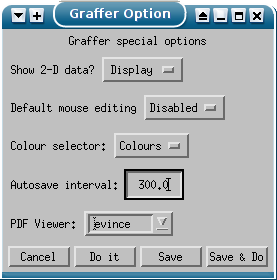
\includegraphics[width=0.5\textwidth]{options}
  \caption{The options menu dialogue.}
  \label{fig:options}
\end{figure}
The ``Options...'' item in the control menu allows you to set a number
of options, via a pop-up dialogue (\textsc{\autoref{fig:options}}).

\begin{description}
\item[Show 2-D data] Toggles the display of 2-D datasets (allows the
  display of contour and image data to be suppressed on slow machines).
\item[Default mouse editing] Controls whether mouse editing is allow on
  new datasets.
\item[Autosave interval] Set the number of seconds between automatic
  saves of the GRAFFER structure.
\item[PDF Viewer] Select the program to use to view the PDF help files.
\end{description}

All these values can be saved to the \texttt{.grafferrc} file in your
home directory, and also applied to the current session (except the
colour selector type).

\subsection{Exit and Help}

The \texttt{Exit} item in the \texttt{File} menu exits from GRAFFER to
the \texttt{IDL>} prompt, it does not exit from IDL. If the file is
changed, you will be given the opportunity to save it or abort the
exit.

The \texttt{Help} button launches a browser to look at a PDF version of
this manual. In addition in the main menu, the text-entry menu, the
hard copy menu and the contour menu a brief description of each
operation appears in a message window when the pointer is moved over a
user-settable item. (IDL does not support help balloons\footnote{No
  longer true, but they are only available for Draw \& Button widgets
  directly in a base widget}.)

\section{Accelerator Keys}
\label{sec:accel}

In version 3.04, accelerator keys were added to the main menu.

The following accelerators are defined:
\begin{description}
\item[Ctrl-Q] Quit.
\item[Ctrl-S] Save.
\item[Ctrl-Shift-S] Save binary as.
\item[Ctrl-Alt-S] Save ascii as.
\item[Ctrl-P] Hard copy -- quick.
\item[Ctrl-Shift-P] Hard Copy -- set up.
\item[Ctrl-N] Open new file.
\item[Ctrl-O] Open existing file.
\item[Ctrl-H] Show user manual.
\item[Ctrl-Alt-P] Dump draw widget to a PNG file.
\item[Ctrl-Alt-T] Dump draw widget to a Tiff file.
\item[Ctrl+Alt+N] Dump draw widget to an Nrfi file.
\end{description}

\section{GRAFF\_ADD (interface user programs to GRAFFER)}
\label{sec:graff_add}

This is all very well but suppose you have a procedure that generates
radial spokes on a series of images and you want to use GRAFFER to make
up a plot of these radial spokes it's going to be rather tedious to
specify all the slices to the top-level variable reader, or write them
to a series of files and then load each file. To automate this and
indeed to allow the use of variables which are never passed back to the
top-level to be used there is a procedure GRAFF\_ADD. GRAFF\_ADD adds
datasets to a GRAFFER file, if need be the file is created, it cannot
delete datasets or replace existing datasets, also some of the more
complex options cannot be set up by GRAFF\_ADD.

N.B. For this an all other programatic \texttt{graffer} tools, you can
check for possible extra keywords by using the command:
\begin{verbatim}
doc_library, 'graff_add'
\end{verbatim}
or whichever routine you want to check at the \texttt{IDL>} prompt.

\subsection{Interface}

\begin{verbatim}
 graff_add, file, [[[z], x,] y, errors=errors, x_func=x_func, $
         y_func=y_func, errtype=errtype, z_func=z_func, $
         polar=polar, rescale=rescale, /display, join=join, $
         style=style, psym=psym, symsize=symsize, colour=colour, $
         thick=thick, neval=neval, description=description, $
         frange=frange, /graffer, /ascii, /noclip, $
         mouse=mouse,z_format=z_format, z_nlevels = z_nlevels, $
         z_levels = $ 
         z_levels, z_colours = z_colours, z_style = z_style, $
         z_thick = z_thick, z_range = z_range, z_label = $
         z_label, z_pxsize = z_pxsize, z_invert = z_invert, $
         z_fill = z_fill, z_log=z_log, z_ctable = z_ctable, $
         xy_file = xy_file, z_file = $
         z_file, func_file = func_file, y_axis=y_axis]
\end{verbatim}

\subsection{Arguments}

\begin{description}
\item[\texttt{file} \textit{string}] The graffer file to modify.
\item[\texttt{z} \textit{float}] The Z values for a 2-D dataset (If
  only 2 arguments are present, then they are treated as X \& Y)
\item[\texttt{x} \textit{float}] The x values to add.
\item[\texttt{y} \textit{float}] The y values to add.
\end{description}



\subsection{Keywords}

\begin{description}
\item[\texttt{errors} \textit{float}] Array with errors, 1-d or (m,n).
\item[\texttt{errtype} \textit{string}] Specify error types as code see
  \textsc{\autoref{ecodes}}
\item[\texttt{x\_func} \textit{string}] Function specification for x =
  f(y) or x = f(t)
\item[\texttt{y\_func} \textit{string}] Function specification for y =
  f(x) or y = g(t)
\item[\texttt{z\_func} \textit{string}] Function specification for z =
  f(x,y)
\item[\texttt{frange} \textit{float}] The range of x, y or t over which
  to plot a function
\item[\texttt{polar} \textit{int}] If unset or 0 rectangular, 1 = polar
  in radians, 2 = polar in degrees.
\item[\texttt{rescale} \textit{flag}] If set, then reset the scaling of
  the plot with the autoscale routine.
\item[\texttt{display} \textit{flag}] If set, then display the plot on
  the current device.
\item[\texttt{style} \textit{int}] The standard IDL linestyle codes
\item[\texttt{psym} \textit{int}] The GRAFFER symbol code - extended
  IDL symbol codes
\item[\texttt{join} \textit{int}] The style of joining: 0 - none, 1 -
  sloping lines, 2 - histogram
\item[\texttt{symsize} \textit{float}] The size for the symbols
  (relative to standard)
\item[\texttt{colour} \textit{int}] Colour number - standard GRAFFER
  colours
\item[\texttt{thick} \textit{float}] Line thickness.
\item[\texttt{neval} \textit{int}] The number of times to evaluate a
  function. (2-elements for \texttt{z\_func})
\item[\texttt{description} \textit{string}] A description of the data
  set.
\item[\texttt{sort} \textit{flag}] Whether to sort the values on the
  X-axis
\item[\texttt{graffer} \textit{flag}] If set, then invoke GRAFFER after
  adding the dataset.
\item[\texttt{ascii} \textit{flag}] If set, then save as an ASCII
  GRAFFER file (default is binary)
\item[\texttt{noclip} \textit{flag}] If set, then disable clipping to
  the axis box.
\item[\texttt{mouse} \textit{int}] If explicitly set to zero then
  disable mouse-editing of the dataset.

\item[\texttt{z\_format} \textit{int}] 2-D datasets, select
  displayformat (0=contour, 1=colour image)

\item[\texttt{z\_nlevels} \textit{int}] For 2D datasets, select number
  of automatic contours

\item[\texttt{z\_levels} \textit{float}] For 2D datasets, select levels
  for explicit contours

\item[\texttt{z\_colours} \textit{int}] For 2D datasets, select the
  colours for the contours

\item[\texttt{z\_style} \textit{int}] For 2D datasets, select
  linestyles for contours

\item[\texttt{z\_thick} \textit{float}] For 2D datasets, select line
  thicknesses for contours

\item[\texttt{z\_label} \textit{int}] Specify the interval of contours
  for labelling.

\item[\texttt{z\_fill} \textit{flag}] If set, then fill the contours.

\item[\texttt{z\_range} \textit{int}] For 2-D datasets, specify the
  cutoff range for image displays

\item[\texttt{z\_pxsize} \textit{float}] For 2D datasets, specify the
  pixel size to use in images for PS device.

\item[\texttt{z\_invert} \textit{flag}] For image display, invert the
  colour table if set.

\item[\texttt{z\_log} \textit{flag}] If set, then map the Z values
  logarithmically.
\item[\texttt{z\_ctable} \textit{int}] Select a colour table for 2-D
  display of images.
\item[\texttt{xy\_file} \textit{string}] A file with a graffer dataset
  (x-y plot).
\item[\texttt{z\_file} \textit{string}] A file with a graffer dataset
  (2-D data).
\item[\texttt{func\_file} \textit{string}] A file with a graffer
  function dataset.
\item[\texttt{y\_axis} \textit{int}] Select which Y-axis to scale this
  data to. (Set but ignored if the file does not have a secondary
  Y-axis).
\end{description}



\subsection{Restrictions}

\begin{itemize}
\item The \texttt{func<xyz>} keys and the x,y,z arguments are
  exclusive.
\item The \texttt{GRAFFER} key overrides the \texttt{DISPLAY} key and
  the \texttt{ASCII} key.
\item There is no support for deleting or replacing datasets.
\end{itemize}


\section{GRAFF\_PROPS (set GRAFFER file properties programmatically)}
\label{sec:graff_props}

This procedure is the global counterpart of \texttt{GRAFF\_ADD}, and
allows you to set various options from your program.\


\subsection{Interface}
\label{sec:gp_interface}

\begin{verbatim}
graff_props, file, title=title, subtitle=subtitle, $
         charsize=charsize, thick=thick, corners=corners, $
         aspect=aspect, comment=comment, xtitle=xtitle, $
         xrange=xrange, xlog=xlog, xexact=xexact, $
         xextend=xextend, xaxes=xaxes, xbox=xbox, $
         xminor=xminor, xtime=xtime, xorigin=xorigin, $
         xgrid=xgrid, xauto=xauto, $
         ytitle=ytitle, $
         yrange=yrange, ylog=ylog, yexact=yexact, $
         yextend=yextend, yaxes=yaxes, ybox=ybox, $
         yminor=yminor, ytime=ytime, yorigin=yorigin, $
         ygrid=ygrid, yauto=yauto, yr_enable = yr_enable, $
         yrtitle=yrtitle, $
         yrrange=yrrange, yrlog=yrlog, yrexact=yrexact, $
         yrextend=yrextend, yraxes=yraxes, $
         yrminor=yrminor, yrtime=yrtime, yrorigin=yrorigin, $
         yrgrid=yrgrid, yrauto=yrauto, display=display, $
         graffer=graffer, ascii=asciih_orient=h_orient, $
         h_colour=h_colour, h_eps=h_eps, h_xsize=h_xsize, $
         h_ysize=h_ysize, h_xmargin=h_xmargin, $
         h_ymargin=h_ymargin isotropic = isotropic, h_cmyk = $
         h_cmyk, ctable = ctable, h_print = h_print, h_viewer $
         = h_viewer, h_file = h_file
\end{verbatim}


\subsection{Arguments}
\label{sec:gp_args}
\begin{description}
\item[\texttt{file} \textit{string}] The graffer file to modify.
\end{description}


\subsection{Keywords}
\label{sec:gp_key}

\begin{description}
\item[\texttt{title} \textit{string}] Set the plot title.
\item[\texttt{subtitle} \textit{string}] Set the subtitle for the plot.
\item[\texttt{charsize} \textit{float}] Set the character size to be
  used for axis labelling and plot annotations.
\item[\texttt{thick} \textit{float}] Set the line thickness to be used
  for drawing the axes.
\item[\texttt{corners} \textit{float}] Set the location of the plot in
  normalized coordinates by specifying the locations of the corners
  (4-elemant array [x0,y0, x1,y1])
\item[\texttt{aspect} \textit{float}] Set the location of the plot
  within the normalized coordinate system by aspect ratio and margin
  (2-element array [aspect, margin] N.B. Specifying both ASPECT \&
  CORNERS is an error and the plot location is unchanged.
\item[\texttt{isotropic} \textit{flag}] Set the plot to use isotropic
  coordinates.
\item[\texttt{comment} \textit{string}] Set a descriptive comment for
  the whole file. (String array)
\item[\texttt{{[x|y|yr]}title} \textit{string}] Set the title for the
  specified axis.
\item[\texttt{{[x|y|yr]}range} \textit{double}] Set the range of the
  specified axis (2-element array).
\item[\texttt{{[x|y|yr]}log} \textit{flag}] Set or unset the use of
  logarithmic axes.
\item[\texttt{{[x|y|yr]}exact} \textit{flag}] Set or unset the exact
  range bit of the IDL axis style setting
\item[\texttt{{[x|y|yr]}extend} \textit{flag}] Set or unset the
  extended range bit of the IDL axis style setting
\item[\texttt{{[x|y|yr]}axes} \textit{flag}] Set or unset the axis
  plotting bit of the IDL axis style setting.
\item[\texttt{{[x|y]}box} \textit{flag}] Set or unset the "box-axis"
  bit in the IDL axis style setting. Note this is not applicable to the
  secondary Y-axis, and is ignored for the main Y-axis if a secondary
  axis is specified.
\item[\texttt{{[x|y|yr]}minor} \textit{flag}] If set, then display
  minor ticks on the plot; if explicitly zero, then turn off the minor
  ticks.
\item[\texttt{{[x|y|yr]}time} \textit{flag/struct}] If set to zero,
  then turn off time labelling, otherwise this must be a structure with
  the members described in \textsc{\autoref{tab:time}}.
  \begin{table}[htbp]
    \centering
    \begin{tabular}{|l|l|}
      \hline
      \texttt{unit}&  0 == seconds\\
      & 1 == minutes\\
      & 2 == hours\\
      & 3 == days\\
      &  Gives the unit in which the\\
      & time is expressed in the axis data.\\
      \hline
      \texttt{max\_unit}& gives the largest unit to\\
      &   display on the plot (same code as\\
      &  for unit)\\
      \hline
      \texttt{zero} & gives the value to be used for \\
      &  the zero of the axis (expressed in\\
      & units of  max\_unit\\
      \hline
    \end{tabular}
    \caption{Time axis structure}
    \label{tab:time}
  \end{table}
\item[\texttt{{[x|y|yr]}origin} \textit{flag}] If set, then plot an
  axis at the origin.
\item[\texttt{{[x|y|yr]}grid} \textit{flag}] Make a grid from the major
  ticks, using linestyle n-1 (0 == no grid).
\item[\texttt{{[x|y|yr]}auto} \textit{flag}] If set, then perform an
  autoscale on the specified axis, the corresponding range setting
  takes precedence over this setting.
\item[\texttt{yr\_enable} \textit{flag}] Enable/disable the display of
  a secondary Y-axis.
\item[\texttt{display} \textit{flag}] If set, then display the plot on
  the current device.
\item[\texttt{graffer} \textit{flag}] If set, then invoke GRAFFER after
  adding the dataset.
\item[\texttt{ascii} \textit{flag}] If set, then save as an ASCII
  GRAFFER file (by default a binary graffer file is generated).
\item[\texttt{h\_orient} \textit{int}] Set landscape(0) or portrait (1)
  orientation of the page.
\item[\texttt{h\_colour} \textit{flag}] Set or unset the generation of
  a colour (E)PS file.
\item[\texttt{h\_cmyk} \textit{flag}] Set or unset the use of the CMYK
  model for (E)PS files. Specifying this keyword will force colour
  (E)PS.
\item[\texttt{h\_eps} \textit{flag}] Set or unset the generation of EPS
  file rather than PS (N.B. if h\_eps is set and h\_orient is not
  specified, then h\_orient=1 is implied).
\item[\texttt{h\_[xy]size} \textit{float}] Set the X(Y) dimension of
  the page in cm
\item[\texttt{h\_[xy]margin} \textit{float}] Set the X(Y) offset of the
  page from the lower-left corner of the page.
\item [\texttt{ctable} \textit{int}] Set the default colour table for
  image display.
\item[\texttt{h\_print} \textit{string(s)}] Specify the command to
  print PS output files (can be a scalar or 2-element aray).
\item[\texttt{h\_viewer} \textit{string(s)}] Specify the command to
  view EPS output files (can be a scalar or 2-element aray).
\item[\texttt{h\_file} \textit{string}] Specify the output file for
  hardcopies.
\end{description}



\subsection{Restrictions}
\label{sec:gp_restrict}

\begin{itemize}
\item The ASPECT and CORNERS keys are exclusive (if both are given,
  both are ignored).

\item {[X|Y|YR]}RANGE overrides {[X|Y|YR]}AUTO.

\item The GRAFFER key overrides the DISPLAY key and the ASCII key.

\item As yet the addition/modification of a key (legend) is not
  supported.

\item Not all hardcopy options can be set.

\end{itemize}


\section{GRAFF\_PRINT (Make a hard copy of a GRAFFER file)}
\label{sec:gh}


\subsection{Interface}
\label{sec:gh_interface}
\begin{verbatim}
        graff_print, file[, <graff_props keywords>]
\end{verbatim}


\subsection{Argument}
\label{sec:gh_args}

\begin{description}
\item[\texttt{file} \textit{string}] The graffer file to modify.
\end{description}


\subsection{Keywords}
\label{sec:gh_key}

Any keyword accepted by \texttt{GRAFF\_PROPS}
(See~\textsc{\autoref{sec:gp_key}}) can be used.

\section{GRAFF\_UPDATE}
\label{sec:graff_update}


User-callable interface to update the properties of a dataset.

\subsection{Interface}
\label{sec:upd_interface}


\begin{verbatim}
graff_update, file, idx, name=name, polar = polar, rescale = rescale, $
            style = style, psym = psym, join = $
            join, symsize = symsize, colour = colour, thick = $
            thick, neval = neval, description = description, $
            sort = sort, ascii = ascii, noclip = noclip, $
            mouse = mouse, z_format = z_format, z_nlevels = $
            z_nlevels, z_levels = z_levels, z_colours = z_colours, $
            z_style = z_style, z_thick = z_thick, z_range = $
            z_range, z_label = z_label, z_pxsize = z_pxsize, $
            z_invert = z_invert, z_fill = z_fill, z_log = z_log, $
            z_ctable = z_ctable, y_axis=y_axis, $
            make_current = make_current x_values = x_values, $
            y_values = y_values, z_values = z_values, x_func = $
            x_func, y_func = y_func, z_func = z_func, xy_file = $ $
            xy_file, z_file = z_file, errors = errors, errtype = $
            errtype, neval = neval, frange = frange
\end{verbatim}

\subsection{Arguments:}
\label{sec:gu_args}


\begin{description}
\item[\texttt{file} \textit{string}] The graffer file to modify.
\item[\texttt{idx} \textit{int}] input The dataset index to modify
  (starting at 1).
\end{description}

\subsection{Keywords:}
\label{sec:gu-keywords}

\begin{description}
\item[\texttt{name} \textit{string}] Find the dataset to update by
  searching the descriptor fields to match the name.
\item[\texttt{frange} \textit{float}] The range of x, y or t over which
  to plot a function
\item[\texttt{polar} \textit{int}] If unset or 0 rectangular, 1 = polar
  in radians, 2 = polar in degrees.
\item[\texttt{rescale} \textit{input}] set, then reset the scaling of
  the plot with the autoscale routine.
\item[\texttt{style} \textit{int}] The standard IDL linestyle codes
\item[\texttt{psym} \textit{int}] The GRAFFER symbol code - extended
  IDL symbol codes.
\item[\texttt{join} \textit{int}] The style of joining: 0 - none 1 -
  sloping lines 2 - histogram
\item[\texttt{symsize} \textit{float}] The size for the symbols
  (relative to standard)
\item[\texttt{colour} \textit{int}] Colour number - standard GRAFFER
  colours (which may well not work on current device).
\item[\texttt{thick} \textit{float}] Line thickness.
\item[\texttt{neval} \textit{int}] The number of times to evaluate a
  function. (2-elements for z\_func)
\item[\texttt{description} \textit{str}] A description of the data set.
\item[\texttt{sort} \textit{input}] to sort the values on the X axis.
\item[\texttt{ascii} \textit{input}] set, then save as an ASCII GRAFFER
  file (by default a binary graffer file is generated).
\item[\texttt{noclip} \textit{input}] set, then disable clipping to the
  axis box.
\item[\texttt{mouse} \textit{int}] If explicitly set to zero then
  disable mouse-editing of the dataset.
\item[\texttt{z\_format} \textit{int}] For 2-D datasets, select display
  format (0=contour, 1=colour image)
\item[\texttt{z\_nlevels} \textit{int}] For 2D datasets, select number
  of automatic contours
\item[\texttt{z\_levels} \textit{float}] For 2D datasets, select levels
  for explicit contours
\item[\texttt{z\_colours} \textit{int}] input For 2D datasets, select
  the colours for the contours
\item[\texttt{z\_style} \textit{int}] For 2D datasets, select
  linestyles for contours
\item[\texttt{z\_thick} \textit{float}] For 2D datasets, select line
  thicknesses for contours
\item[\texttt{z\_label} \textit{int}] Specify the interval of contours
  for labelling.
\item[\texttt{/z\_fill}] If set, then fill the contours.
\item[\texttt{z\_range} \textit{int}] For 2-D datasets, specify the
  cutoff range for image displays
\item[\texttt{z\_pxsize} \textit{float}] For 2D datasets, specify the
  pixel size to use in images for PS device.
\item[\texttt{/z\_invert}] For image display, invert the colour table
  if set.
\item[\texttt{/z\_log}] If set, then map the Z values logarithmically.
\item[\texttt{z\_ctable} \textit{int}] Select a colour table for 2-D
  display of images.
\item[\texttt{y\_axis} \textit{int}] Select to which Y-axis the dataset
  will be scaled.
\item[\texttt{/make\_current}] If set, then make the modified dataset
  into the current dataset when the file is next opened.
\item[\texttt{x\_values} \textit{double}] New X values.
\item[\texttt{y\_values} \textit{double}] New Y values.
\item[\texttt{z\_values} \textit{double}] New Z values.
\item[\texttt{x\_func} \textit{string}] New x=f(y), or x=f(t)
\item[\texttt{y\_func} \textit{string}] New y=f(x), or y=f(t).
\item[\texttt{z\_func} \textit{string}] New z=f(x,y).
\item[\texttt{xy\_file} \textit{string}] File for new 1-D data.
\item[\texttt{z\_file} \textit{string}] File for new 2-D data.
\item[\texttt{errors} \textit{double}] New error values.
\item[\texttt{errtype} \textit{string}] Specify error types as code
  (e.g. "XXY" for asymmetrical errors in X and symmetric errors in Y)
\item[\texttt{frange} \texttt{float}] The range of x, y or t over which
  to plot a function
\end{description}

\subsection{Restrictions:}
\label{sec:gu-restr}

Does not allow the type of dataset to be changed.  If neither the index
or the name is given, then the current dataset is modified.  Specifying
both is an error.  If name is given then (1) If there are 2 datasets of
the same name, the first will be modified, (2) if the name is not
found, then the program exits without updating.

\section{GRAFF\_EXPORT}
\label{sec:graff_export}


\begin{verbatim}
graff_export, file, index, name = name, outfile = outfile
\end{verbatim}

\subsection{Arguments}
\label{sec:ge-args}

\begin{description}
\item[\texttt{file} \textit{string}] The graffer file.
\item[\texttt{index} \textit{int}] The index of the dataset to write.
\end{description}

\subsection{Keywords}
\label{sec:ge-keys}

\begin{description}
\item[\texttt{name}	\textit{string}] The descriptor of the dataset to write.
\item[\texttt{outfile}	\textit{string}] The file to which to write the dataset
\end{description}

\subsection{Notes}
\label{sec:ge-notes}

If neither the index or the name is given, then the current dataset is
written.  Specifying both is an error.  If name is given then (1) If
there are 2 datasets of the same name, the first will be written, (2)
if the name is not found, then the program exits without writing.

\section{GRAFF\_ANNOTATE}
\label{sec:graff_annotate}

	Add or modify an annotation to a graffer file.

\subsection{Interface}
\label{sec:ga-inter}

\begin{verbatim}
graff_annotate, file[, value, <keywords>]
\end{verbatim}

\subsection{ Arguments}
\label{sec:ga-args}



\begin{description}
\item[\texttt{file} \textit{string}] The file to modify
\item[\texttt{value} \textit{string}] The text of the
  annotation to modify (This is not generally a good way to identify
  the annotation).
\end{description}

 \subsection{Keywords}
 \label{sec:ga-keys}

 \begin{description}
\item[\texttt{id} \textit{string}] The ID tag of the annotation to modify.
\item[\texttt{index} \textit{int}] The index number (1-based) of the annotation
		to modify
\item[\texttt{/substring}] If set, then VALUE may match an initial substring.
\item[\texttt{/case\_squash}] If set, then VALUE is matched without regard
		to case.
\item[\texttt{text} \textit{string}] New text for the annotation.
\item[\texttt{newid} \textit{string}] A new ID for the annotation.
\item[\texttt{colour} \textit{int}] The colour for the annotation.
\item[\texttt{size} \textit{float}] The font size for the annotation
\item[\texttt{orient} \textit{float}] The orientation of the annotation
		(anticlockwise, degrees)
\item[\texttt{align} \textit{float}] The alignment (0=left, 1=right, 0.5=centre)
\item[\texttt{ffamily} \textit{int}] The font group to use (-1 Hershey, 0 hardware,
		1 TrueType)
\item[\texttt{/hershey}] Set Hershey fonts.
\item[\texttt{/truetype}] Set TrueType fonts.
\item[\texttt{/hardware}] Set hardware fonts
\item[\texttt{font} \textit{int}] Set the font index for the desired font.
\item[\texttt{thick} \textit{float}] Set the line thickness for Hershey fonts.
\item[\texttt{x} \textit{float}] Set the X-coordinate of the origin
\item[\texttt{y} \textit{float}] Set the Y-coordinate of the origin
\item[\texttt{norm} \textit{int}] Set the coordinate system, 0=data,
		1=normalized, 2 = "frame".
\item[\texttt{axis} \textit{int}] For data coordinates, set which Y axis to use.
\item[\texttt{status} \textit{int}] A named variable, set to 1 on success, 0 on
		failure.
\item[\texttt{/ascii}] 	If set, then save to an ascii format file.
\end{description}

\subsection{ Notes}
\label{sec:ga-notes}

	The behaviour if more than one font family keyword is set is
	undefined.
	Specifying more than one identification is an error, if no
	identification is given then a new annotation is created.
	For a new annotation, at least TEXT, X and Y must be given

 \section{GRAFF\_GET\_DATA}
 \label{sec:graff-get-data}

 
	Extract data from a graffer file.

 \subsection{Usage:}
 \label{sec:ggd-usage}

 
\begin{verbatim}
graff_get_data, file[, index, <extraction keys>]
\end{verbatim}

\subsection{ Argument:}
\label{sec:ggd-args}

\begin{description}
\item[\texttt{file}	\textit{string}]	The file to extract.

\item[\texttt{idx}	\textit{int}]	The dataset index to extract

\end{description}

\subsection{ Keywords:}
\label{sec:ggd-keys}

\begin{description}
\item[\texttt{name} \textit{string}] Specify the dataset by name.
\item[\texttt{xval} \textit{double}] A variable to contain the X
  values.
\item[\texttt{yval} \textit{double}] A variable to contain the Y
  values.
\item[\texttt{zval} \textit{double}] A variable to contain the Z
  values.
\item[\texttt{xerr} \textit{double}] A variable to contain the X
  errors.
\item[\texttt{yerr} \textit{double}] A variable to contain the Y
  errors.
\end{description}



\subsection*{Acknowledgements}

Thanks to Norbert Hahn of the University of Darmstadt for suggesting
the need for a more compact format for those using the package on small
screens. And to Christian Marquand of the Free University of Berlin for
providing a fix to the plot symbol pixmaps for little-endian
machines. To Phil Williams of the Children's Hospital Medical Center,
Cincinnati OH for suggesting the revisions of the compact format. To
Simon Plunkett of USRA for the idea of the alternate key format. To Tim
Howard of SwRI for the idea of adjusting font sizes in the key.

\appendix

\section{Useful procedures}

This is a quick list of some of the procedures that are part of GRAFFER
which are likely to be of use in other contexts, they are mostly
compound widgets which offer some extensions over the versions in the
IDL User's library:

\begin{description}
\item[cw\_pdmenu\_plus] An extended pulldown menu. Compared with the
  supplied \texttt{cw\_pdmenu} this offers a number of extra
  facilities:
  \begin{itemize}
  \item Tracking events that identify which menu item is entered.
  \item Stateful buttons, including the option to create a group with
    exclusive selection.
  \item Bitmap buttons. Currently, all buttons must use bitmaps or all
    buttons must use strings. Also for monochrome bitmaps, the number
    of columns must be a multiple of 8.
  \item A \texttt{cw\_bselector} or \texttt{widget\_droplist} like
    mode, allowing desensitized menu items.
  \end{itemize}
\item [graff\_enter]An entry box with rather more options than
  CW\_FIELD (e.g. format, capture focus on pointing, tracking events).
\item [fractile]Return specified percentiles of an array of values.
\end{description}
For more details, use the DOC\_LIBRARY procedure. There may be other
useful routines that I've missed.

\section{\texttt{.grafferrc}}
\label{sec:grafferrc}

The \texttt{.grafferrc} file provides a very limited range of control
over the default settings for GRAFFER. It is a colon-separated text
file with just five options.
\begin{description}
\item[\texttt{Autosave:} \textit{float}] The time between autosave
  operations in seconds. (300.)
\item[\texttt{Supp2D:} \textit{bool}] Whether to suppress display of
  2-D datasets (for slow machines, really a legacy of the
  mid-90's whne GRAFFER was first developed). (0)
\item[\texttt{MouseEdit:} \textit{bool}] Whether to enable mouse
  editing of data by default. (0)
\item[\texttt{PDFView:} \textit{string}] The program to use to view the
  PDF help files. (searches for the first of \texttt{acroread},
  \texttt{kpdf}, \texttt{xpdf}, \texttt{kghostview}, \texttt{gv},
  \texttt{okular} and \texttt{evince} to be installed)
\end{description}
The usual way to create and modify it is via the \textsf{Options} menu
(\textsc{\autoref{sec:options}}) by selecting \textsf{Save} or \textsf{Save
  and Do}.

\section{X Resources (X windows systems only)}

All the top-level widget bases in GRAFFER have the key
\texttt{resource='Graffer'} specified. This allows the user to specify
colours for GRAFFER widgets that are different from this of other IDL
widgets. Putting the following into your \texttt{.Xdefaults} makes
{}``lemon yellow'' GRAFFER widgets and light green widgets for other
IDL widgets .

\begin{verbatim}
  ! This sets the number of colors IDL reserves.
  ! Leave 5 unallocated color
  ! table entries for other applications and 
  ! the windowing system:

  Idl.colors:     -5
  Idl*background: palegreen
  Idl*text*background: lightcyan
  Idl*button*background: lightcyan
  Idl*slider*background: lightcyan
  Idl*list*background: lightcyan
  Idl*droplist*background: lightcyan

  ! These are specific to Graffer

  Idl*Graffer*background: \#ffff88
  Idl*Graffer*text*background: white
  Idl*Graffer*button*background: white
  Idl*Graffer*slider*background: white
  Idl*Graffer*list*background: white
\end{verbatim}

\end{document}
